‌\section{Introducción}
Con este diseño se busca un sistema de venta de telefonía celular que permita tener un alto grado de confiabilidad tanto para el vendedor como para el cliente, que mantenga interconectadas a las distintas partes de la empresa (marketing - ventas - facturación - stock) en todo momento, que automatice algunos procesos internos de la empresa y que agilice y mejore el rendimiento de ventas.\\

\section{Diagrama de Contexto}

En estos diagramas presentamos de contexto presentamos los agentes que 
involucran el sistema a diseñar y cómo interactúan entre sí.

\subsection{Alternativa 1}

En esta primer alternativa las acciones que realiza el sistema son minimales. El 
sistema actúa primariamente como una base de datos que mantiene el estado del 
stock, promociones, ventas y facturación dependiendo.

Si bien esta alternativa parece ser poco útil, nos parece importante notarla 
como la herramienta más chica que resuelve el problema, dado que se puede presentar 
al cliente como el MVP (Minimum Viable Product) al partir del cual evolucionar.

\begin{figure}[h!]
  \centering
  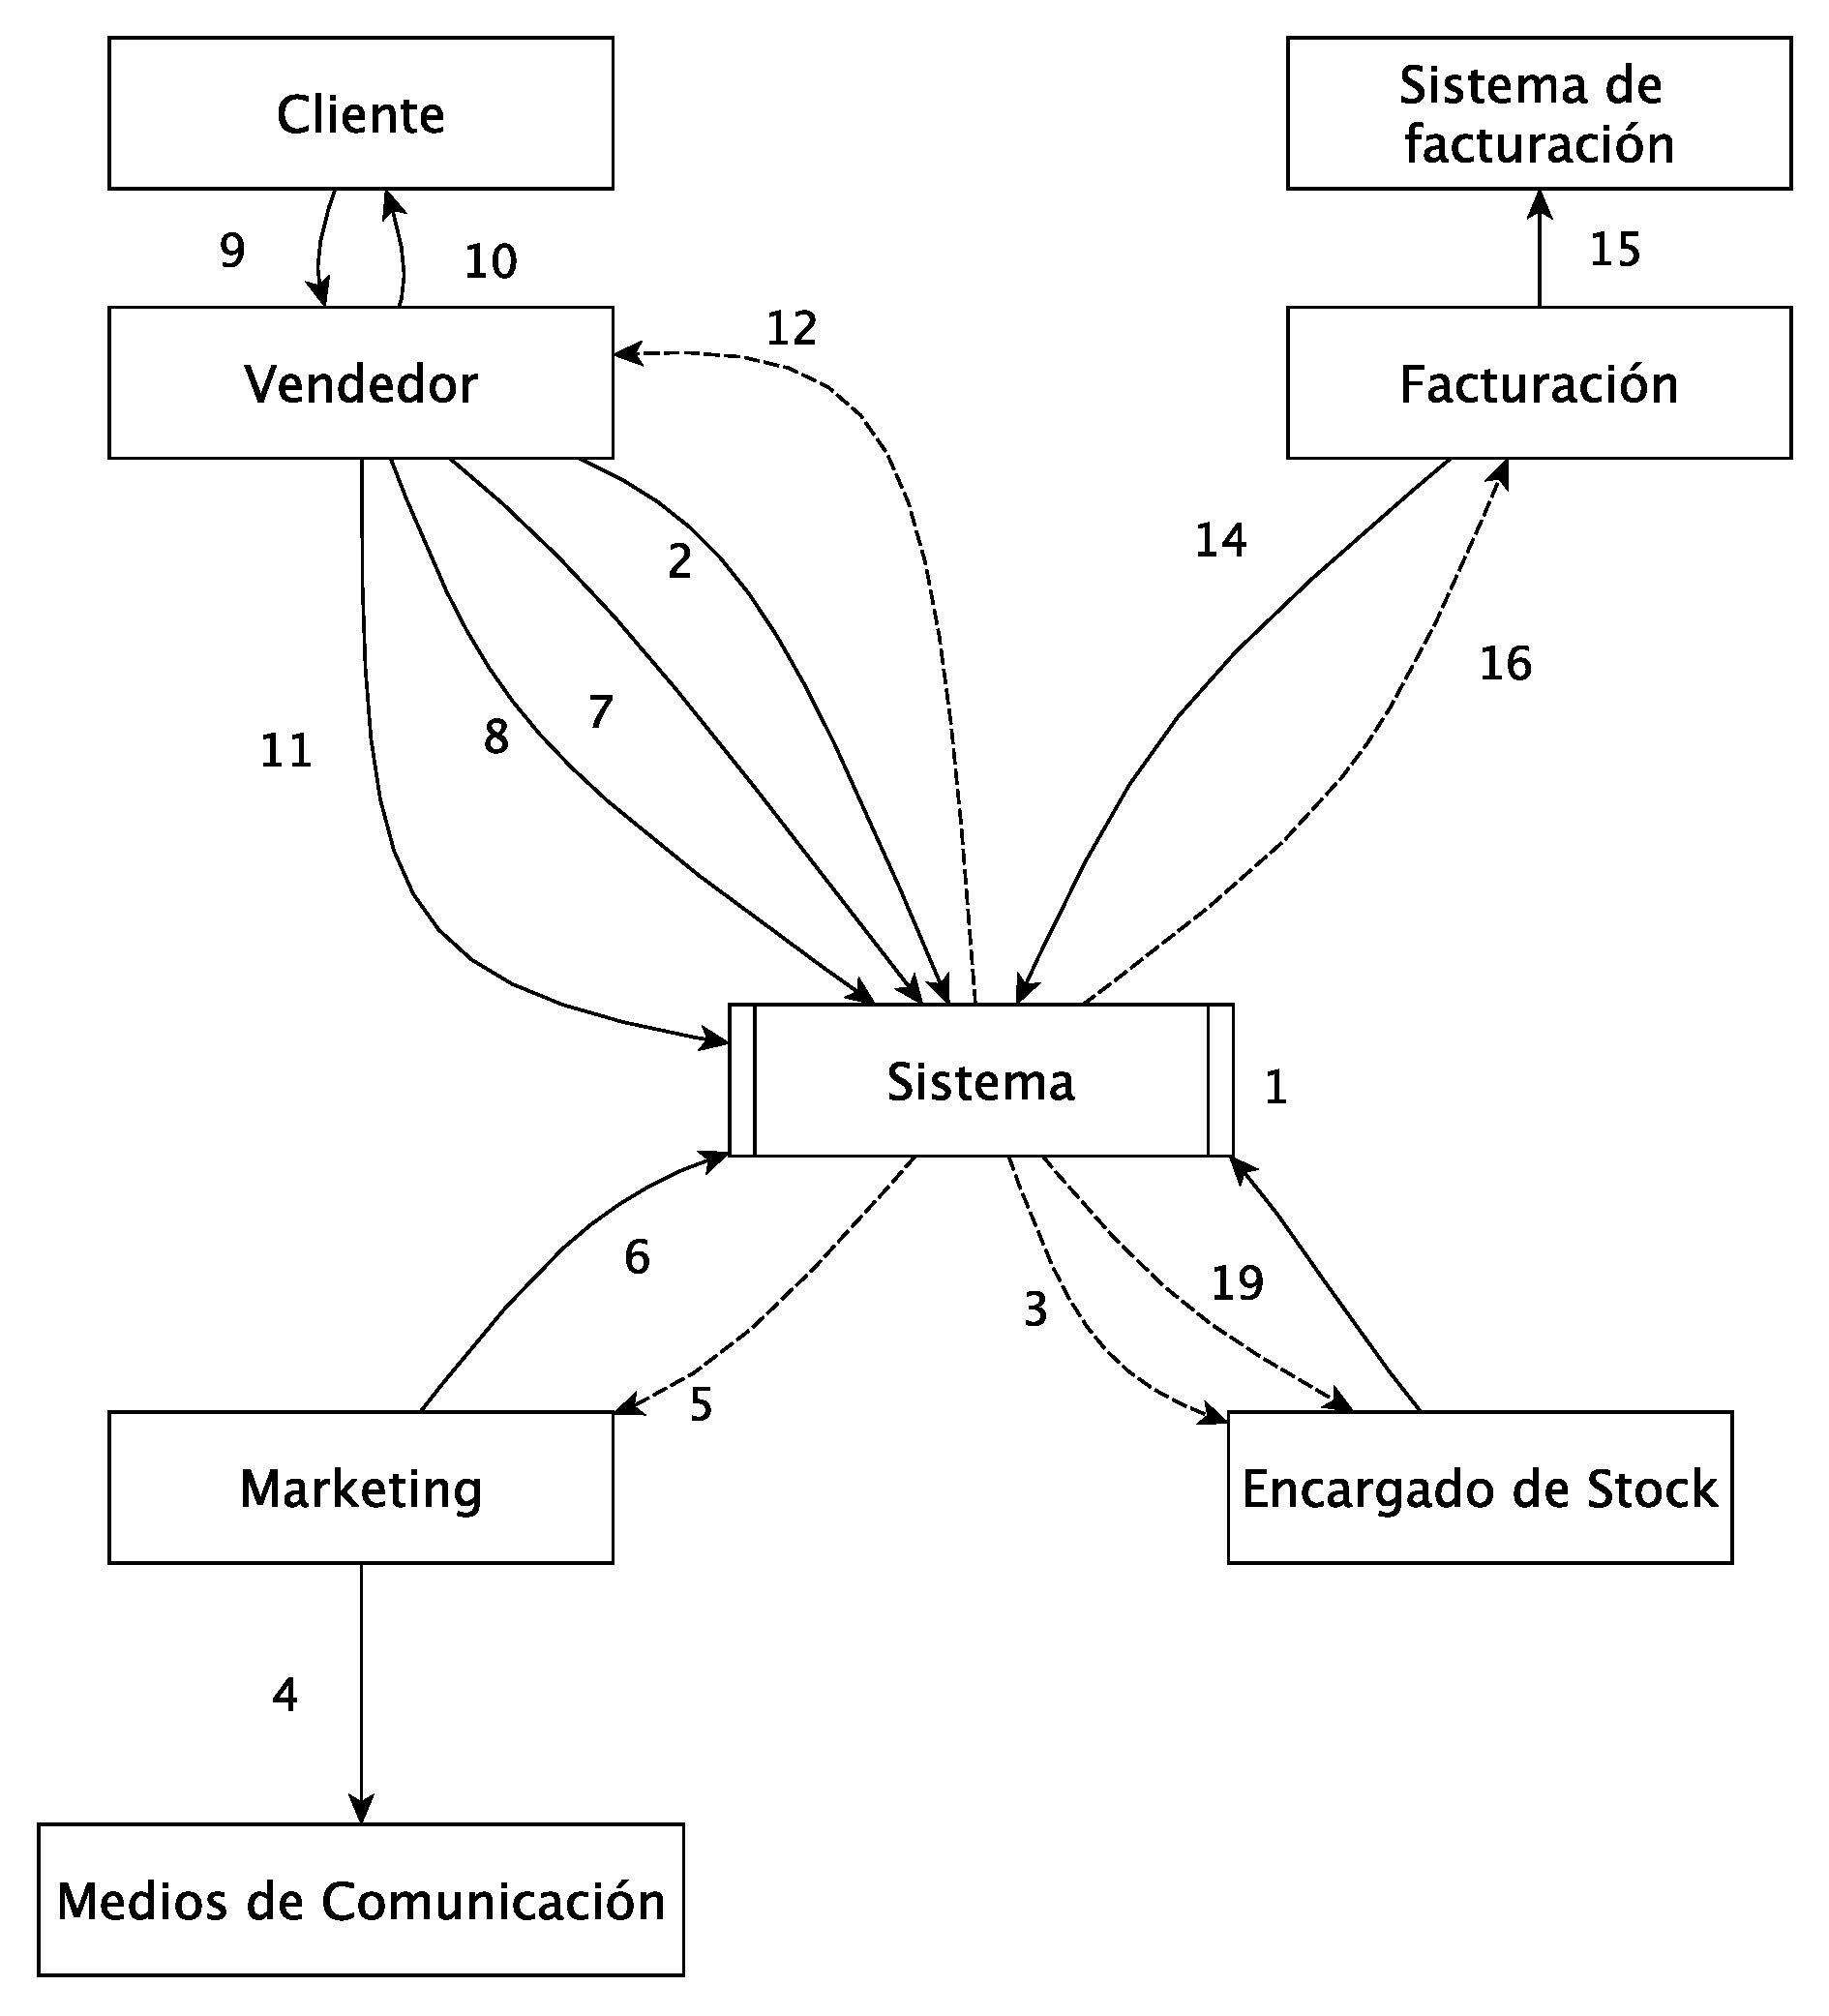
\includegraphics[width=0.5\textwidth]{./imagenes/contexto_2.pdf}
  \caption{Diagrama de Contexto para Sistema de Venta de Celulares (MVP)}
\end{figure}

\subsection{Eventos}

\begin{enumerate}

  \item Ingresar nuevos equipos.
  \item Registrar o cancelar reserva de equipos.
  \item Notificar la confirmación de reserva de equipos.
  \item Monitorear los medios de comunicación.
  \item Notificar stock acumulado.
  \item Dar alta o baja nueva promoción.
  \item Actualizar datos de clientes.
  \item Actualizar promociónes para clientes.
  \item Comunicar necesidades.
  \item Convencer de adquirir promoción.
  \item Seleccionar la promoción adquirida por el cliente.
  \item Confirmar o rechazar promoción por disponibilidad de stock.
  \item Alertar cuando stock está pronto a acabarse.
  \item Confirmar o rechazar venta.
  \item Cargar la venta de los equipos y las líneas.
  \item Notificar venta nueva para ser verificada.

\end{enumerate}

\subsection{Alternativa 2}

En esta segunda opción damos más responsabilidades al sistema para asistir a los 
diferentes departamentos, por ejemplo, realizando un monitoreo de internet para 
favorecer el conocimiento del mercado, o la creación automática de posibles 
promociones basadas en el stock y el análisis del mercado.

\begin{figure}[h!]
  \centering
  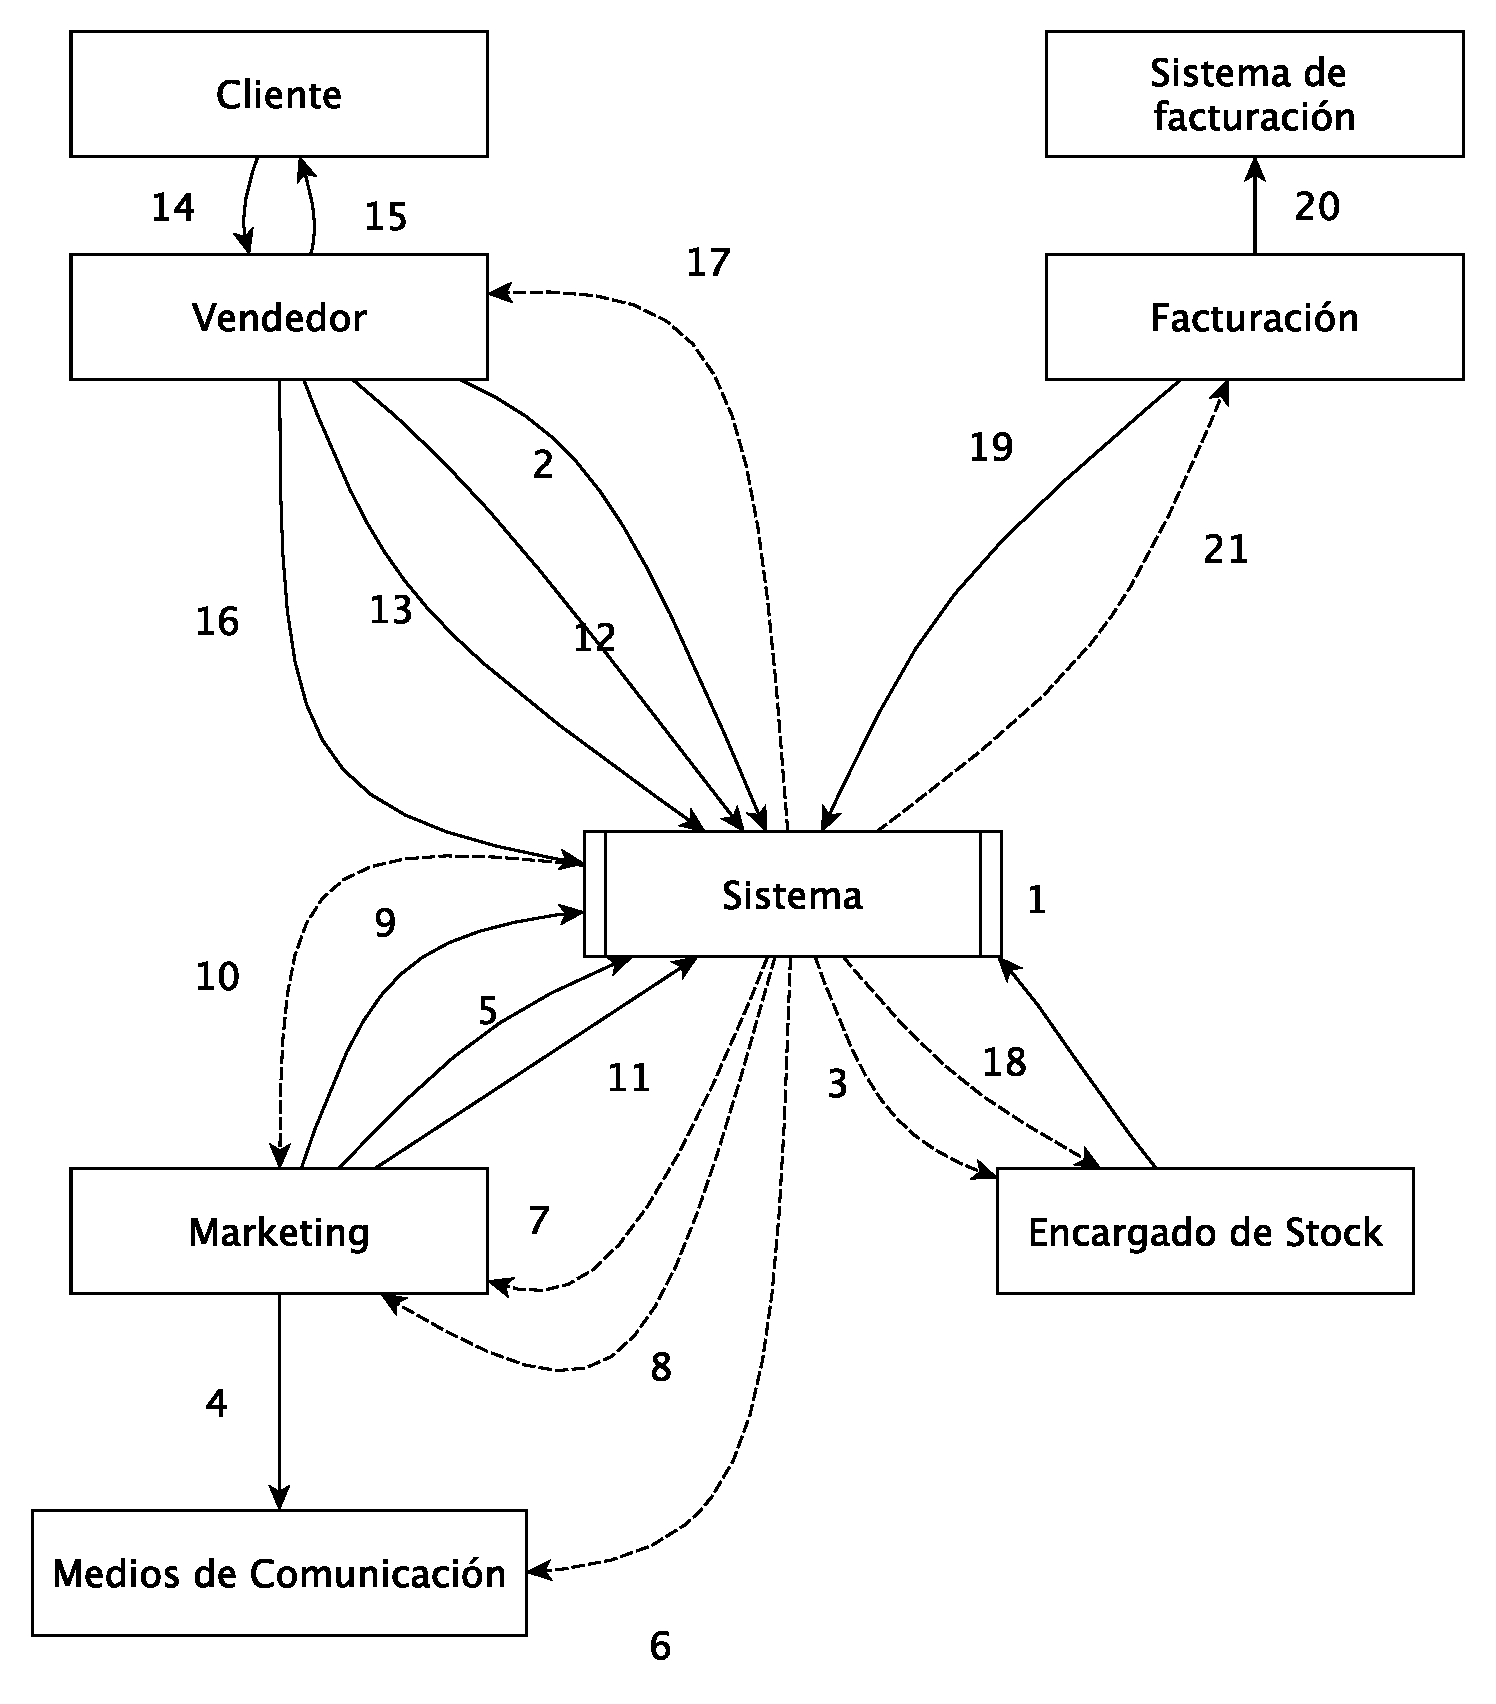
\includegraphics[width=0.5\textwidth]{./imagenes/contexto_1.pdf}
  \caption{Diagrama de Contexto para Sistema de Venta de Celulares}
\end{figure}

\subsection{Eventos}

\begin{enumerate}

  \item Ingresar nuevos equipos.
  \item Registrar o cancelar reserva de equipos.
  \item Notificar la confirmación de reserva de equipos.
  \item Monitorear los medios tradicionales de comunicación.
  \item Seleccionar usuarios y sitos a monitorear.
  \item Monitorear competencia por internet.
  \item Enviar informe de estado del mercado.
  \item Notificar que se creó promoción automáticamente. (vale para mercacdo y stock acumulado)
  \item Validar promoción creada automátiacmente. (vale para mercacdo y stock acumulado)
  \item Notificar stock acumulado.
  \item Dar alta o baja nueva promoción.
  \item Consultar en el momento datos del cliente.
  \item Consultar en el momento promociónes para el cliente.
  \item Comunicar necesidades.
  \item Convencer de adquirir promoción.
  \item Seleccionar la promoción adquirida por el cliente.
  \item Confirmar o rechazar promoción por disponibilidad de stock.
  \item Alertar cuando stock está pronto a acabarse.
  \item Confirmar o rechazar venta.
  \item Cargar la venta de los equipos y las líneas.
  \item Notificar venta nueva para ser verificada.

\end{enumerate}

\clearpage


\section{Diagrama de objetivos}

Para la presentación del diagrama de objetivos decidimos fraccionar el mismo en sus cuatro ramas principales, las cuales componen los aspectos más importantes del diseño del sistema según lo antes descrito. En la figura ~\ref{fig:diagGen} presentamos el nivel superior del diagrama, donde construimos el objetivo principal en base a estos cuatro pilares. Para lograr llevar adelante el sistema que proponemos debemos garantizar, por un lado, poder controlar el stock con precisión y de manera actualizada, registrando ingresos y egresos y, principalmente, evitando problemas de concurrencia entre vendedores actuando al mismo tiempo. Además se deben poder diseñar y cargar con ayuda del software diseñado promociones atractivas para los clientes, no sólo en base a su historia dentro de la empresa sino también en consonancia con el mercado global. Será primordial en el aspecto operativo lograr una venta eficiente y automatizada, donde el vendedor pueda verse desligado de cualquier inconveniente técnico para así poder enfocarse en satisfacer al cliente. Por último, la integración del proceso de venta al sistema informatizado de facturación ayudará a eliminar el esfuerzo y el error humano a la hora de ingresar, contabilizar y facturar las ventas realizadas.

\begin{figure}[h!]
  \centering
  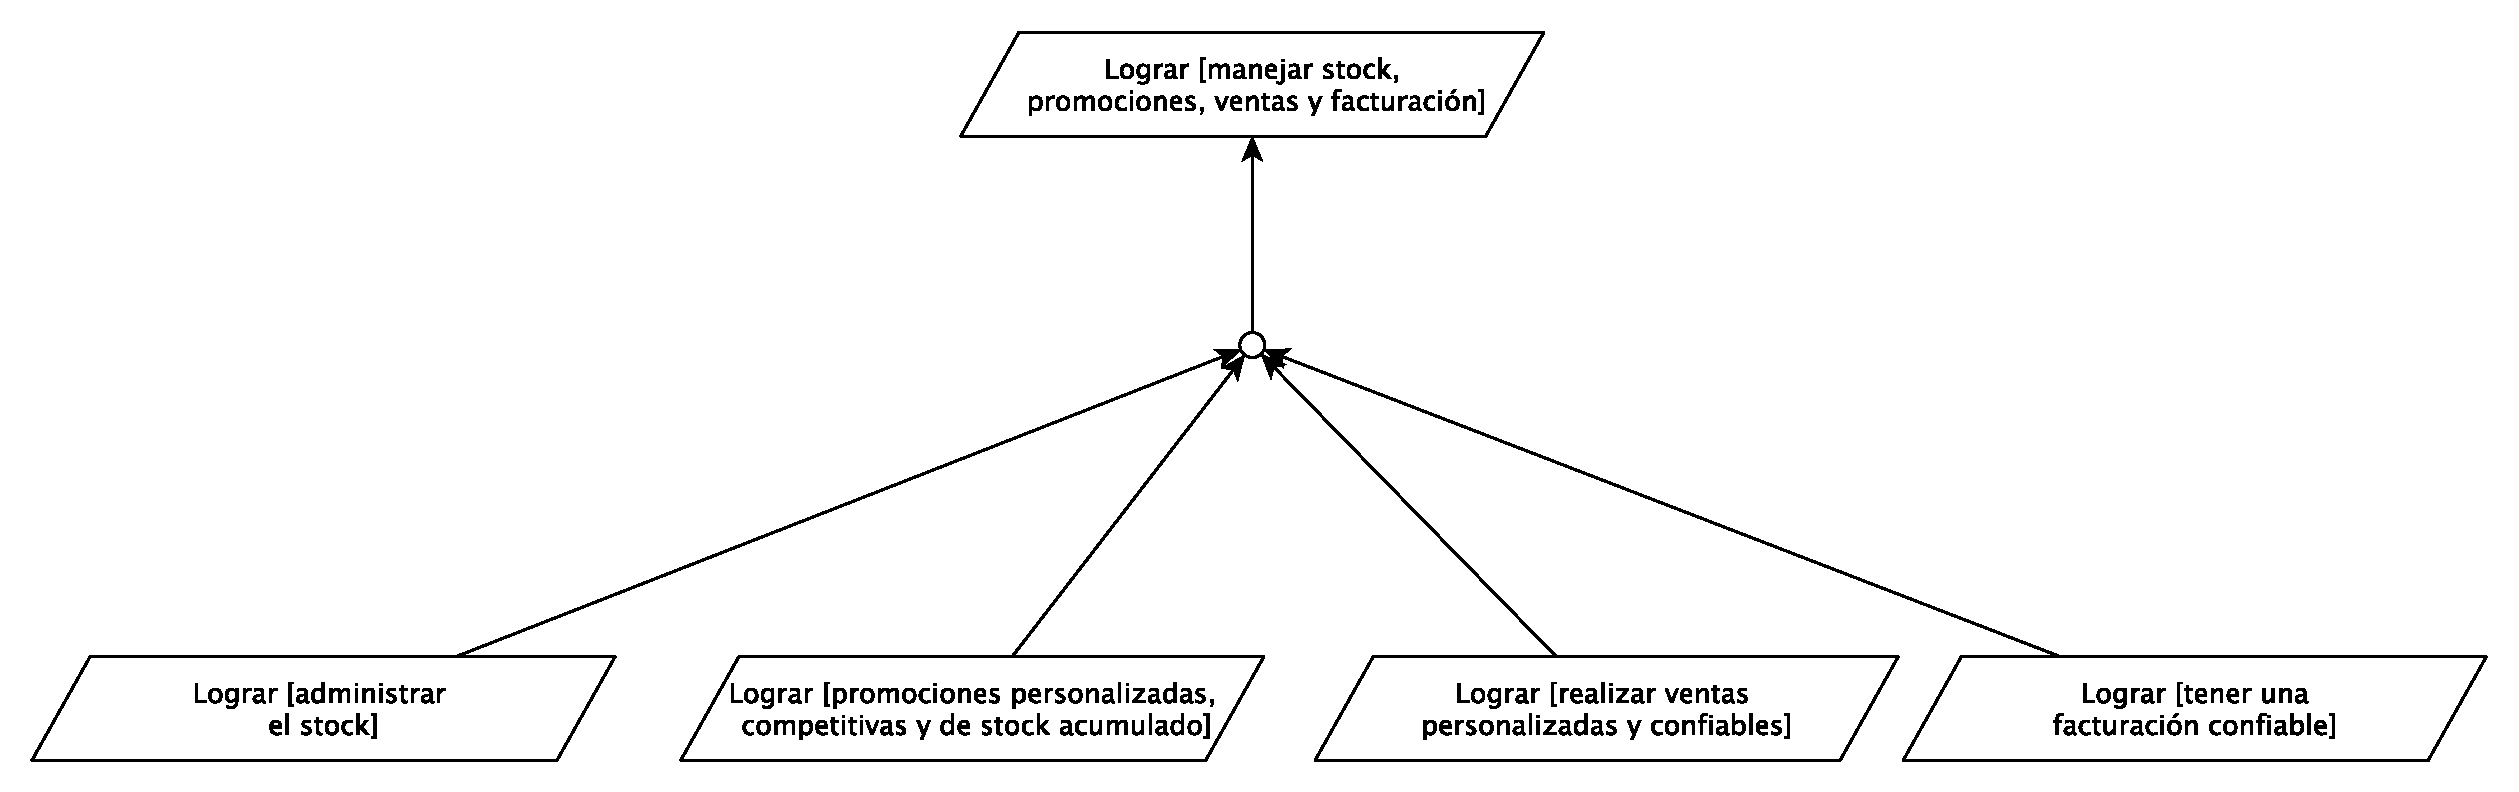
\includegraphics[width=1\textwidth]{./imagenes/general_top.pdf}
  \caption{Diagrama de objetivos - General}
  \label{fig:diagGen}
\end{figure}


\subsection{Rama Stock}

\begin{figure}[h!]
  \centering
  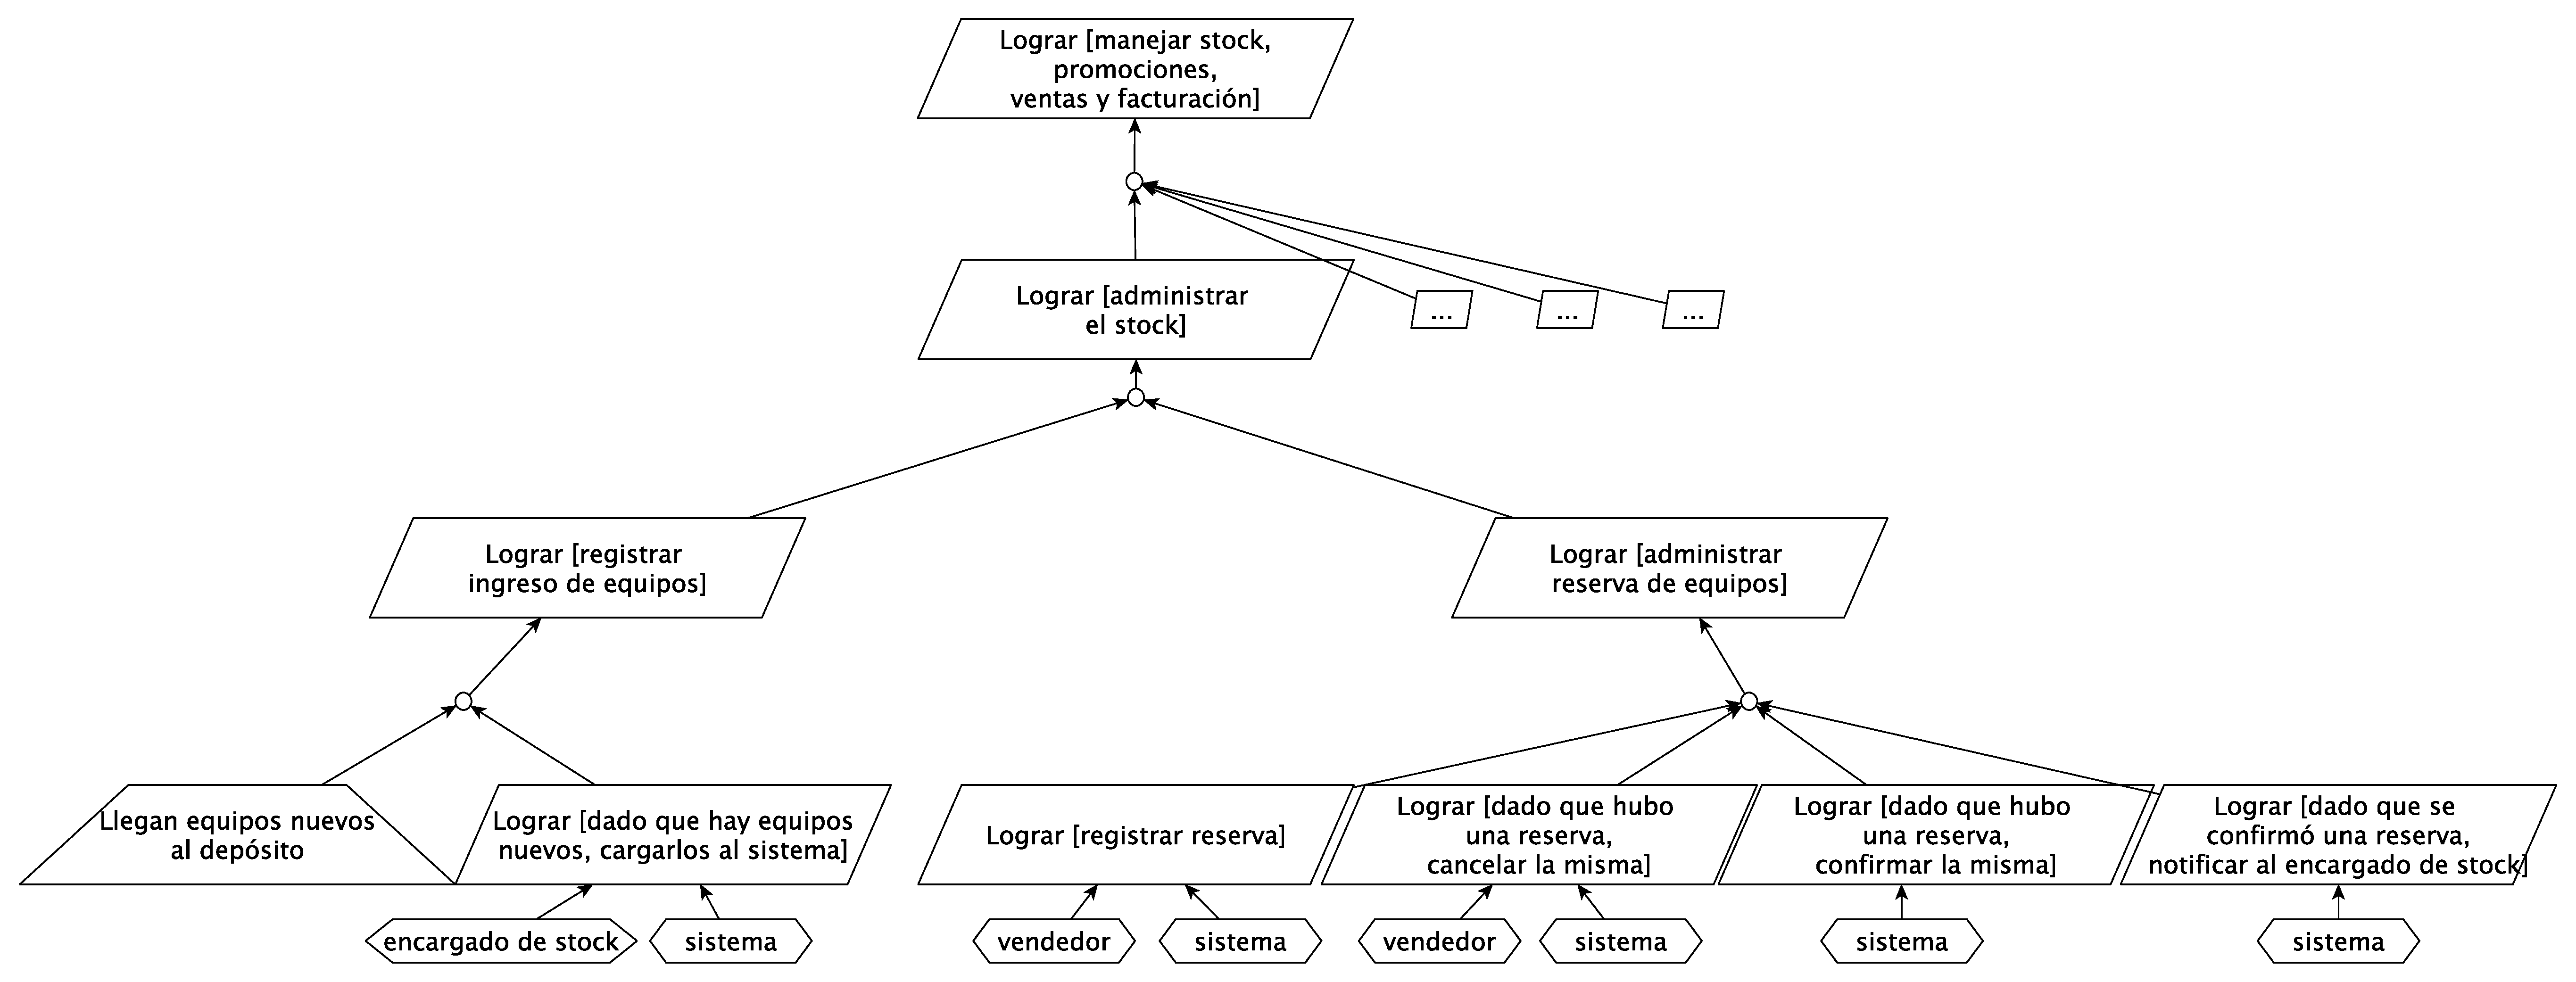
\includegraphics[width=1\textwidth]{./imagenes/stock.pdf}
  \caption{Diagrama de objetivos - Stock}
  \label{fig:diagStock}
\end{figure}

La figura ~\ref{fig:diagStock} presenta la rama de objetivos referente al manejo de stock. La administración del mismo se basa en dos puntos: registrar el ingreso de mercadería nueva y manejar la reserva (y eventual egreso) de los equipos que se vendan. Es importante notar la diferencia entre reserva y venta efectiva (que luego devendrá en egreso del depósito hacia el cliente). Durante la visita del vendedor a un cliente, si éste se decidiera por adquirir una promoción, el vendedor procederá a reservar la misma. Si la reserva le es concedida (ver Rama Ventas), tendrá una ventana de tiempo para confirmar o cancelar la misma. En caso de confirmarla, se le envía una notificación al encargado de stock pero de todas maneras éste deberá aguardar a la notificación de facturación, una vez que la venta haya sido ratificada por el departamento. En caso de cancelación, se restituye la cantidad de stock que se había sacado de circulación al otorgar la reserva para que otros vendedores puedan disponer de esa mercadería. Es importante señalar que la notificación de reserva permite al departamento de stock llevar una cuenta más detallada y controlada del flujo de equipos en sus distintas etapas, a la vez que permite mediante la automatización evitar en un alto grado la disposición errónea de equipos. \\
\indent El control del ingreso de dispositivos móviles es más sencillo y se basa fundamentalmente en la presunción de dominio de que los equipos encargados arriban al depósito en tiempo y forma. Luego, el sistema deberá proveer de una interfaz para que el encargado de stock pueda registrar ese ingreso de manera que esté disponible no sólo para el equipo de ventas sino también para que marketing lance las promociones asociadas con aquellos equipos que sean nuevos y no existieran previamente en el catálogo de la empresa.

\subsubsection{Escenarios}

\begin{itemize}
  \item \textbf{Ingreso de equipos}
    Estéban, el encargado de stock, recibe los nuevos equipos en el depósito y los ingresa en el sistema utilizando la interfaz del mismo.
  \item \textbf{Egreso de equipos}
    Cuando se produce una venta efectiva, el sistema genera una notificación y Estéban debe entregar los equipos al cliente y marcarlos como retirados en el sistema.
\end{itemize}

\subsection{Rama Promociones}

El subárbol de objetivos correspondiente a las promociones fue dividido en dos partes. Satisfacer este aspecto del sistema se basa en cuatro pilares: por un lado lograr promociones parametrizadas y promociones competitivas, objetivos que se exploran en la figura ~\ref{fig:diagProm1}. Por el otro, generar promociones de stock acumulado y mantener actualizado y coherente el catálogo de promociones, metas que se muestran en la figura ~\ref{fig:diagProm2}. En lo que respecta a promociones parametrizadas, este objetivo ataca la necesidad de tener una oferta atractiva para los distintos perfiles de clientes. Gracias a que el sistema lleva cuenta de sus clientes y su historia de consumo, marketing dispone de la información necesaria para crear categorías de clientes en base a la cantidad de líneas que poseen y el dinero que gastan en determinado período y en base a esto generar promociones de acuerdo a los parámetros de estos perfiles. De esta manera, los vendedores podrán optar por consultar promociones a medida del tipo de cliente que visitan de una manera eficiente y rápida.\\
\indent Desde otro enfoque también es importante que las promociones tengan correlación con el estado del mercado y que resulten competitvas respecto de otras empresas de telefonía celular. Para esto deberá conocerse el mercado y luego diseñar ofertas acorde a las conclusiones obtenidas. Aquí se presentan por primera vez alternativas sobre cómo abordar un aspecto del sistema. El alcance del estudio de mercado podrá ser en base a internet o además también en base a los medios de comunicación tradicionales como diarios, revistas, radio, etc. Si bien esta última esfera de comunicación sólo podrá ser analizada manualmente por marketing, una de las alternativas que se ofrece es poder llevar adelante un monitoreo automático de internet (y no manual). A simple vista se puede reflexionar que incorporar al sistema una funcionalidad automática de escaneo del mercado en internet será más costoso y no necesariamente más eficiente que hacerlo de manera manual pero deberá tenerse en cuenta también que permitirá una reacción muy rápida frente a cambios en el mercado para contrarrestar a los competidores. En ese caso, marketing deberá primero definir cierto alcance de la búsqueda como ser sitios, redes sociales, usuarios y canales virtuales de difusión de la empresa. Luego, el sistema procederá a procesar toda esa información y a generar un reporte que será enviado a marketing para su desglose.\\
\indent Una vez que marketing cuenta con el estado de mercado, el objetivo inmediato a satisfacer es la correcta creación de promociones en base a esta información. Nuevamente se ofrecen dos alternativas: la creación manual de las mismas, a cargo de marketing, o una creación automática por parte del sistema pero sujeta a revisión por un agente humano de marketing. Esta vez la disyuntiva es similar, puesto que incorporar un módulo de creación automática de promociones seguramente será más costoso, pero por otro lado si para el estudio de mercado se decidió realizarlo automáticamente, podría impactar en menor medida en el costo del segundo sistema automático dado que podría procesar de manera eficiente el reporte emitido en el primer paso. Además, con el uso cada vez mayor de las redes sociales e internet para la difusión de promociones y ofertas por parte de las companías, a largo plazo podría resultar muy ventajoso y liberador de recursos humanos contar con autogeneración de promociones competitivas.\\
\indent El diseño del sistema no pierde de vista que el objetivo principal de la empresa, en otras palabras, es la rentabilidad. Por eso un objetivo importante que deberá cumplirse es el de la generación de promociones de stock acumulado, es decir, de aquellos conjuntos de equipos que superen cierto número en depósito y sea mejor tratar de despacharlos antes de que se vuelvan obsoletos. Dado que se cumple la administración de stock, el sistema ya cuenta con un monitoreo sumamente actualizado de la mercadería. Según un umbral de alerta definido por el equipo de marketing, el sistema alertará al mismo cuando cierto modele supere ese valor. Otra vez se podrá optar por que marketing diseñe las promociones acordes en este caso de manera manual o que el sistema se encargue y luego marketing las valide. En este caso, la alternativa automatizada no será tan costosa puesto que ya se cuenta con el monitoreo de stock y el tipo de oferta podrá ser parametrizada de antemano por marketing sin mucho problema. De esta manera se ahorrará tiempo y trabajo humano para lograr comercializar de manera efectiva el excedente de mercadería. Por último, es de vital importancia que se pueda regular el catálogo de promociones de manera que se puedan publicar nuevas y no circulen promociones desactualizadas. Todo esto se llevará a cabo mediante una interfaz entre sistema y marketing, lo cual le posibilitará estas acciones al equipo en cuestión.

\subsubsection{Escenarios}

\begin{itemize}
  \item \textbf{Promociones parametrizadas} \\
    Martín, de Marketing, consulta en el sistema la cantidad de líneas que posee el cliente y el consumo del mismo. Luego, utiliza esta información para categorizarlo.
    Al mismo tiempo, el departamento de Marketing trabaja en promociones basadas en las categorías de los clientes.

  \item \textbf{Promociones competitivas}
  \begin{itemize}
    \item \textbf{Conocer el estado del mercado - Automaticamente} \\
      Martín y el resto del equipo de Marketing ingresan en el sistema las páginas de interes de donde sacar información de la competencia, ya sean redes sociales, blogs, diarios e inclusive las mismas páginas de la competencia. El sistema fue desarrollado para obtener información valiosa de estos sitios donde luego de técnicas de DataMining genera un reporte que es enviado al departamento de Marketing.
    \item \textbf{Conocer el estado del mercado - Manualmente} \\
      Martín, Manuel, Miriam y Marisol revisan periodicamente las redes sociales, blogs, diarios y páginas de la competencia para elaborar el reporte que necesita Marketing para poder diseñar promociones competitivas.
    \item \textbf{Conocer el estado del mercado - Híbrido} \\
      Manuel y Marisol revisan periodicamente las páginas de la competencia y blogs, mientras que a la par el sistema obtiene información de las redes sociales seleccionadas y en conjunto elaborar un reporte final que será necesario por el departamento de Marketing para elaborar las nuevas promociones competitivas.
  \end{itemize}

  \begin{itemize}
    \item \textbf{Crear promociones en base al reporte - Manualmente} \\
      Miriam y Marisol analizan el reporte sobre el estado del mercado, discuten y diseñan nuevas promociones.
    \item \textbf{Crear promociones en base al reporte - Automaticamente y Verificarlas} \\
      El sistema parte de la información obtenida en el reporte y diseña algunas promociones similares a las de la competencia.
      Luego de generarlas, el equipo de Marketing es notificado sobre las promociones diseñadas y es este equipo quien las verifíca.
  \end{itemize}

  \item \textbf{Promociones de Stock acumulado} \\
    El sistema mantiene actualizado el inventario de la empresa y registro de los movimientos de cada equipo. Cuando el sistema detecta que bajan las ventas de determinados equipos o se empieza a acumular en el depósito, éste notifica al departamento de Marketing para crear promociones con estos equipos.
  \begin{itemize}
    \item \textbf{Crear promociones - Manualmente} \\
      Manuel y Miriam comienzan a diseñar una promoción con los equipos acumulados y la cargan en el sistema.
    \item \textbf{Crear promociones - Automaticamente y Verificarlas} \\
      El sistema propone algunas promociones creadas por el mismo y son Miriam y Manuel los que verifícan las promociones.
  \end{itemize}

  \item \textbf{Actualizar la lista de promociones vigentes} \\
    El equipo de Marketing da de alta las promociones elaboradas y verificadas que se encuentran en el sistema. Éste mismo equipo revisa la lista de promociones del sistema y se encarga de eliminar las promociones que quedaron desactualizadas u obsoletas.

\end{itemize}

\clearpage

\begin{figure}[h!]
  \centering
  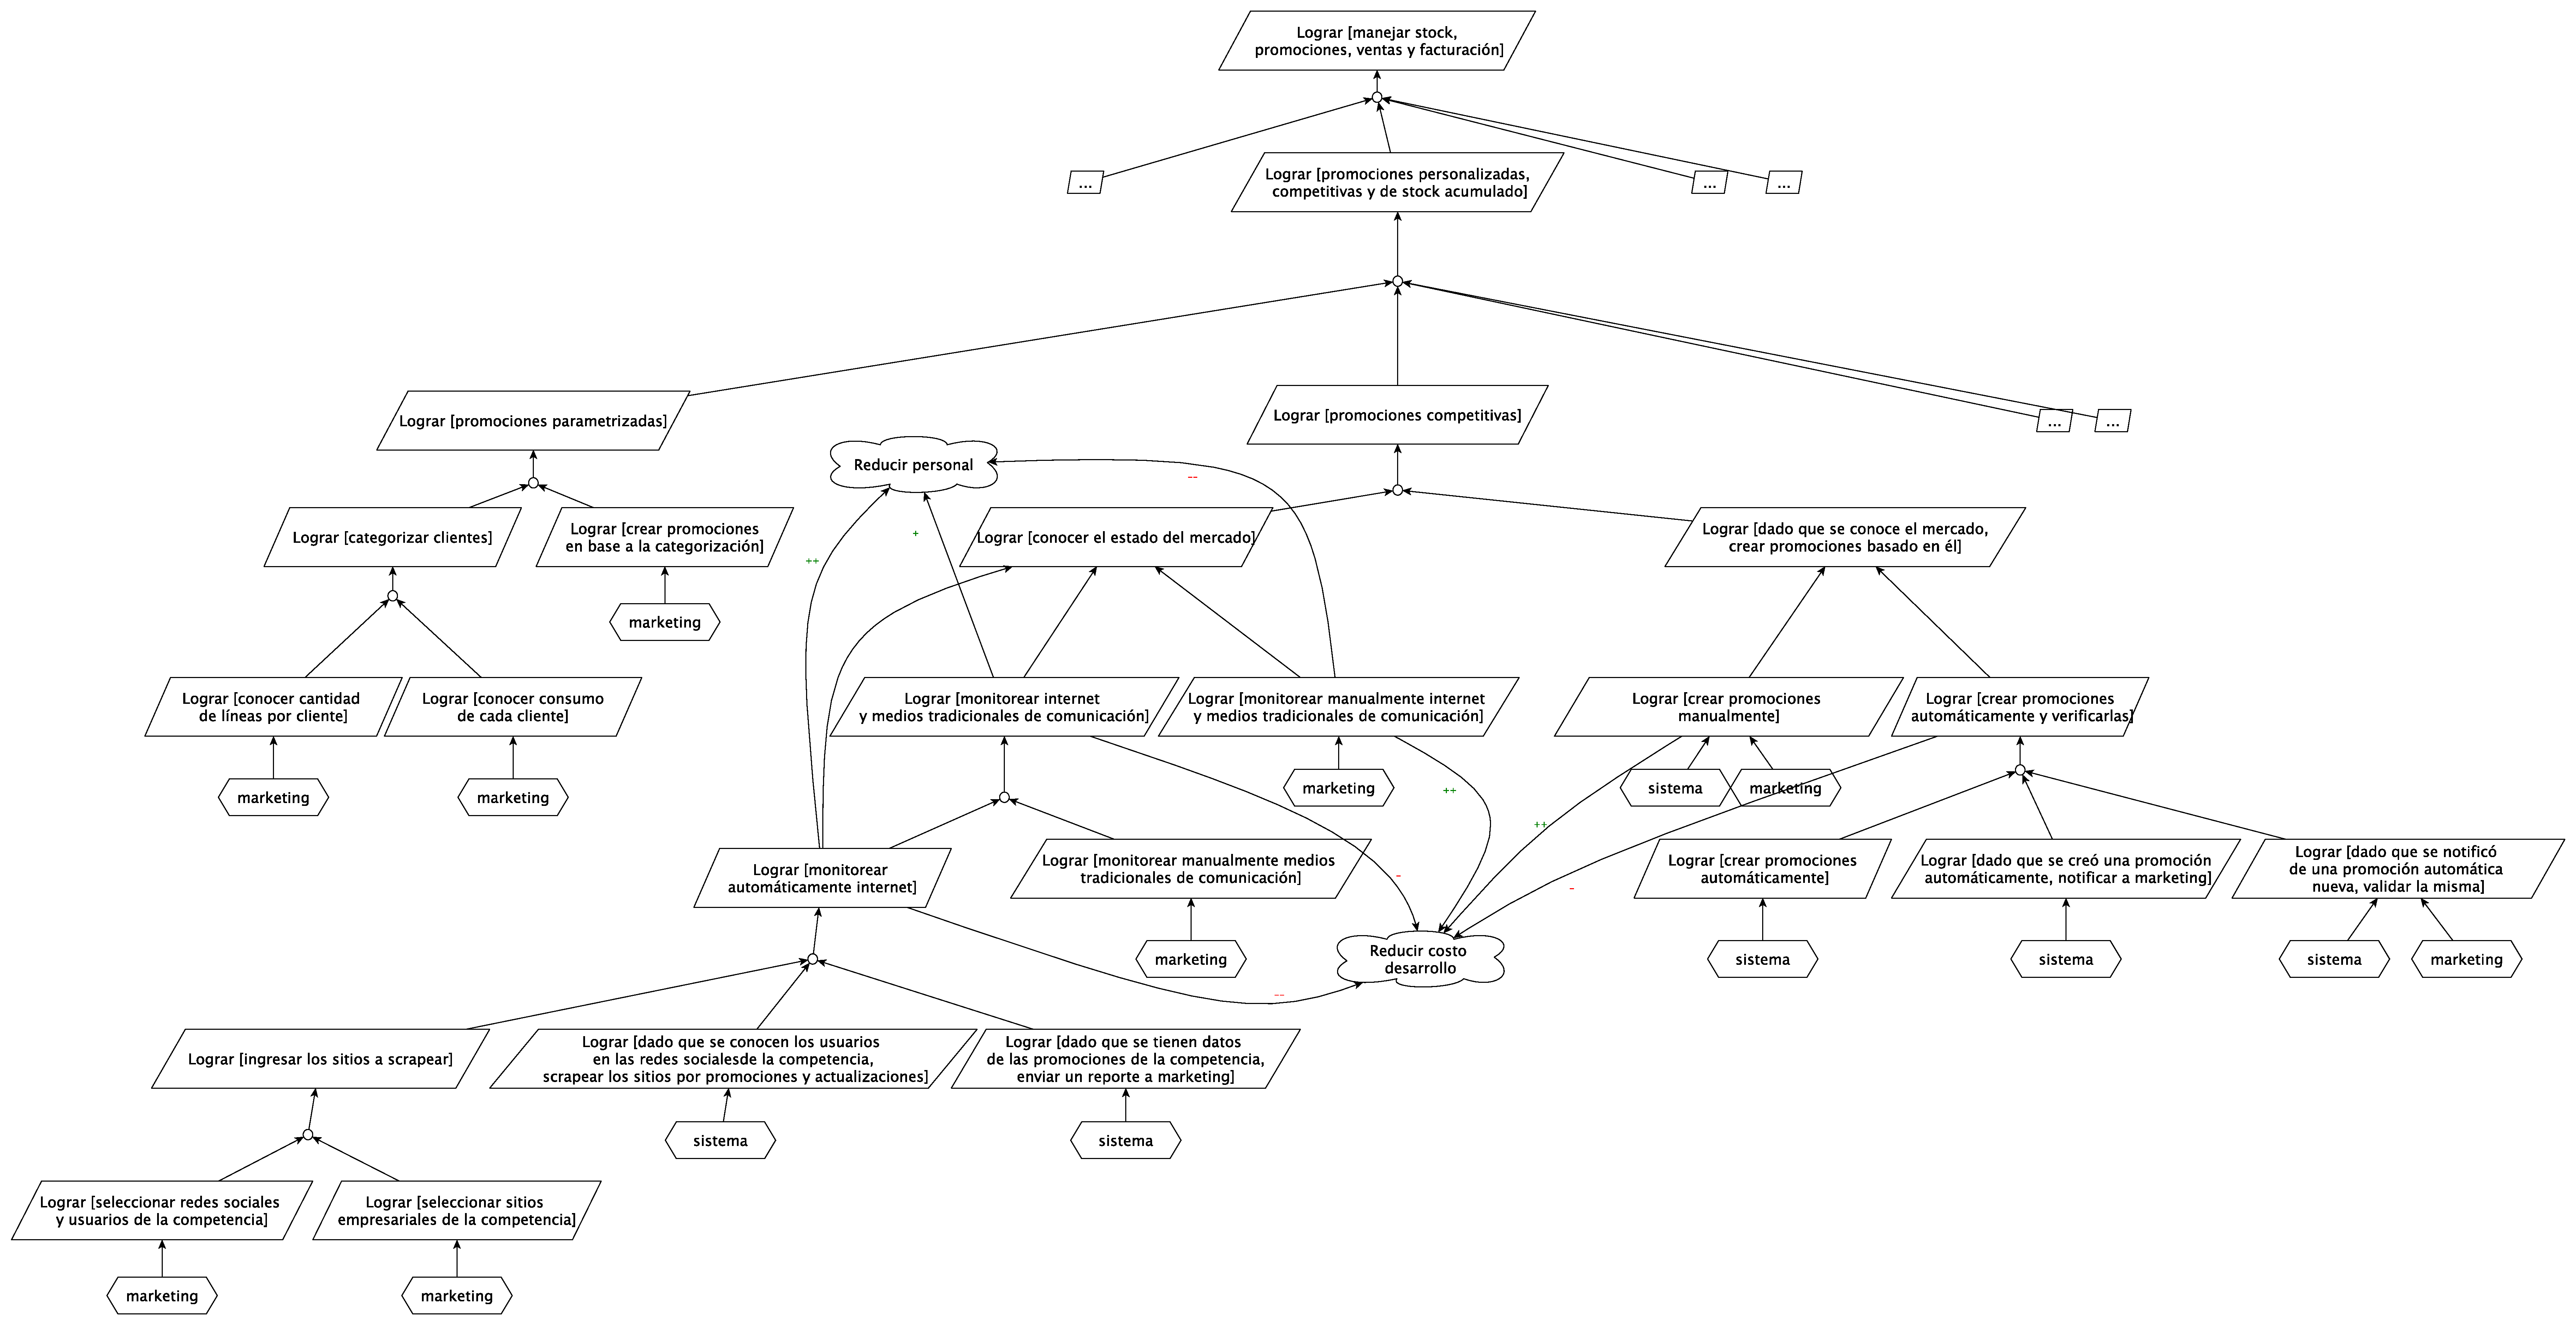
\includegraphics[width=1.5\textwidth, angle=90]{./imagenes/promociones_1.pdf}
  \caption{Diagrama de objetivos - Promociones (parte 1)}
  \label{fig:diagProm1}
\end{figure}

\clearpage


\begin{figure}[h!]
  \centering
  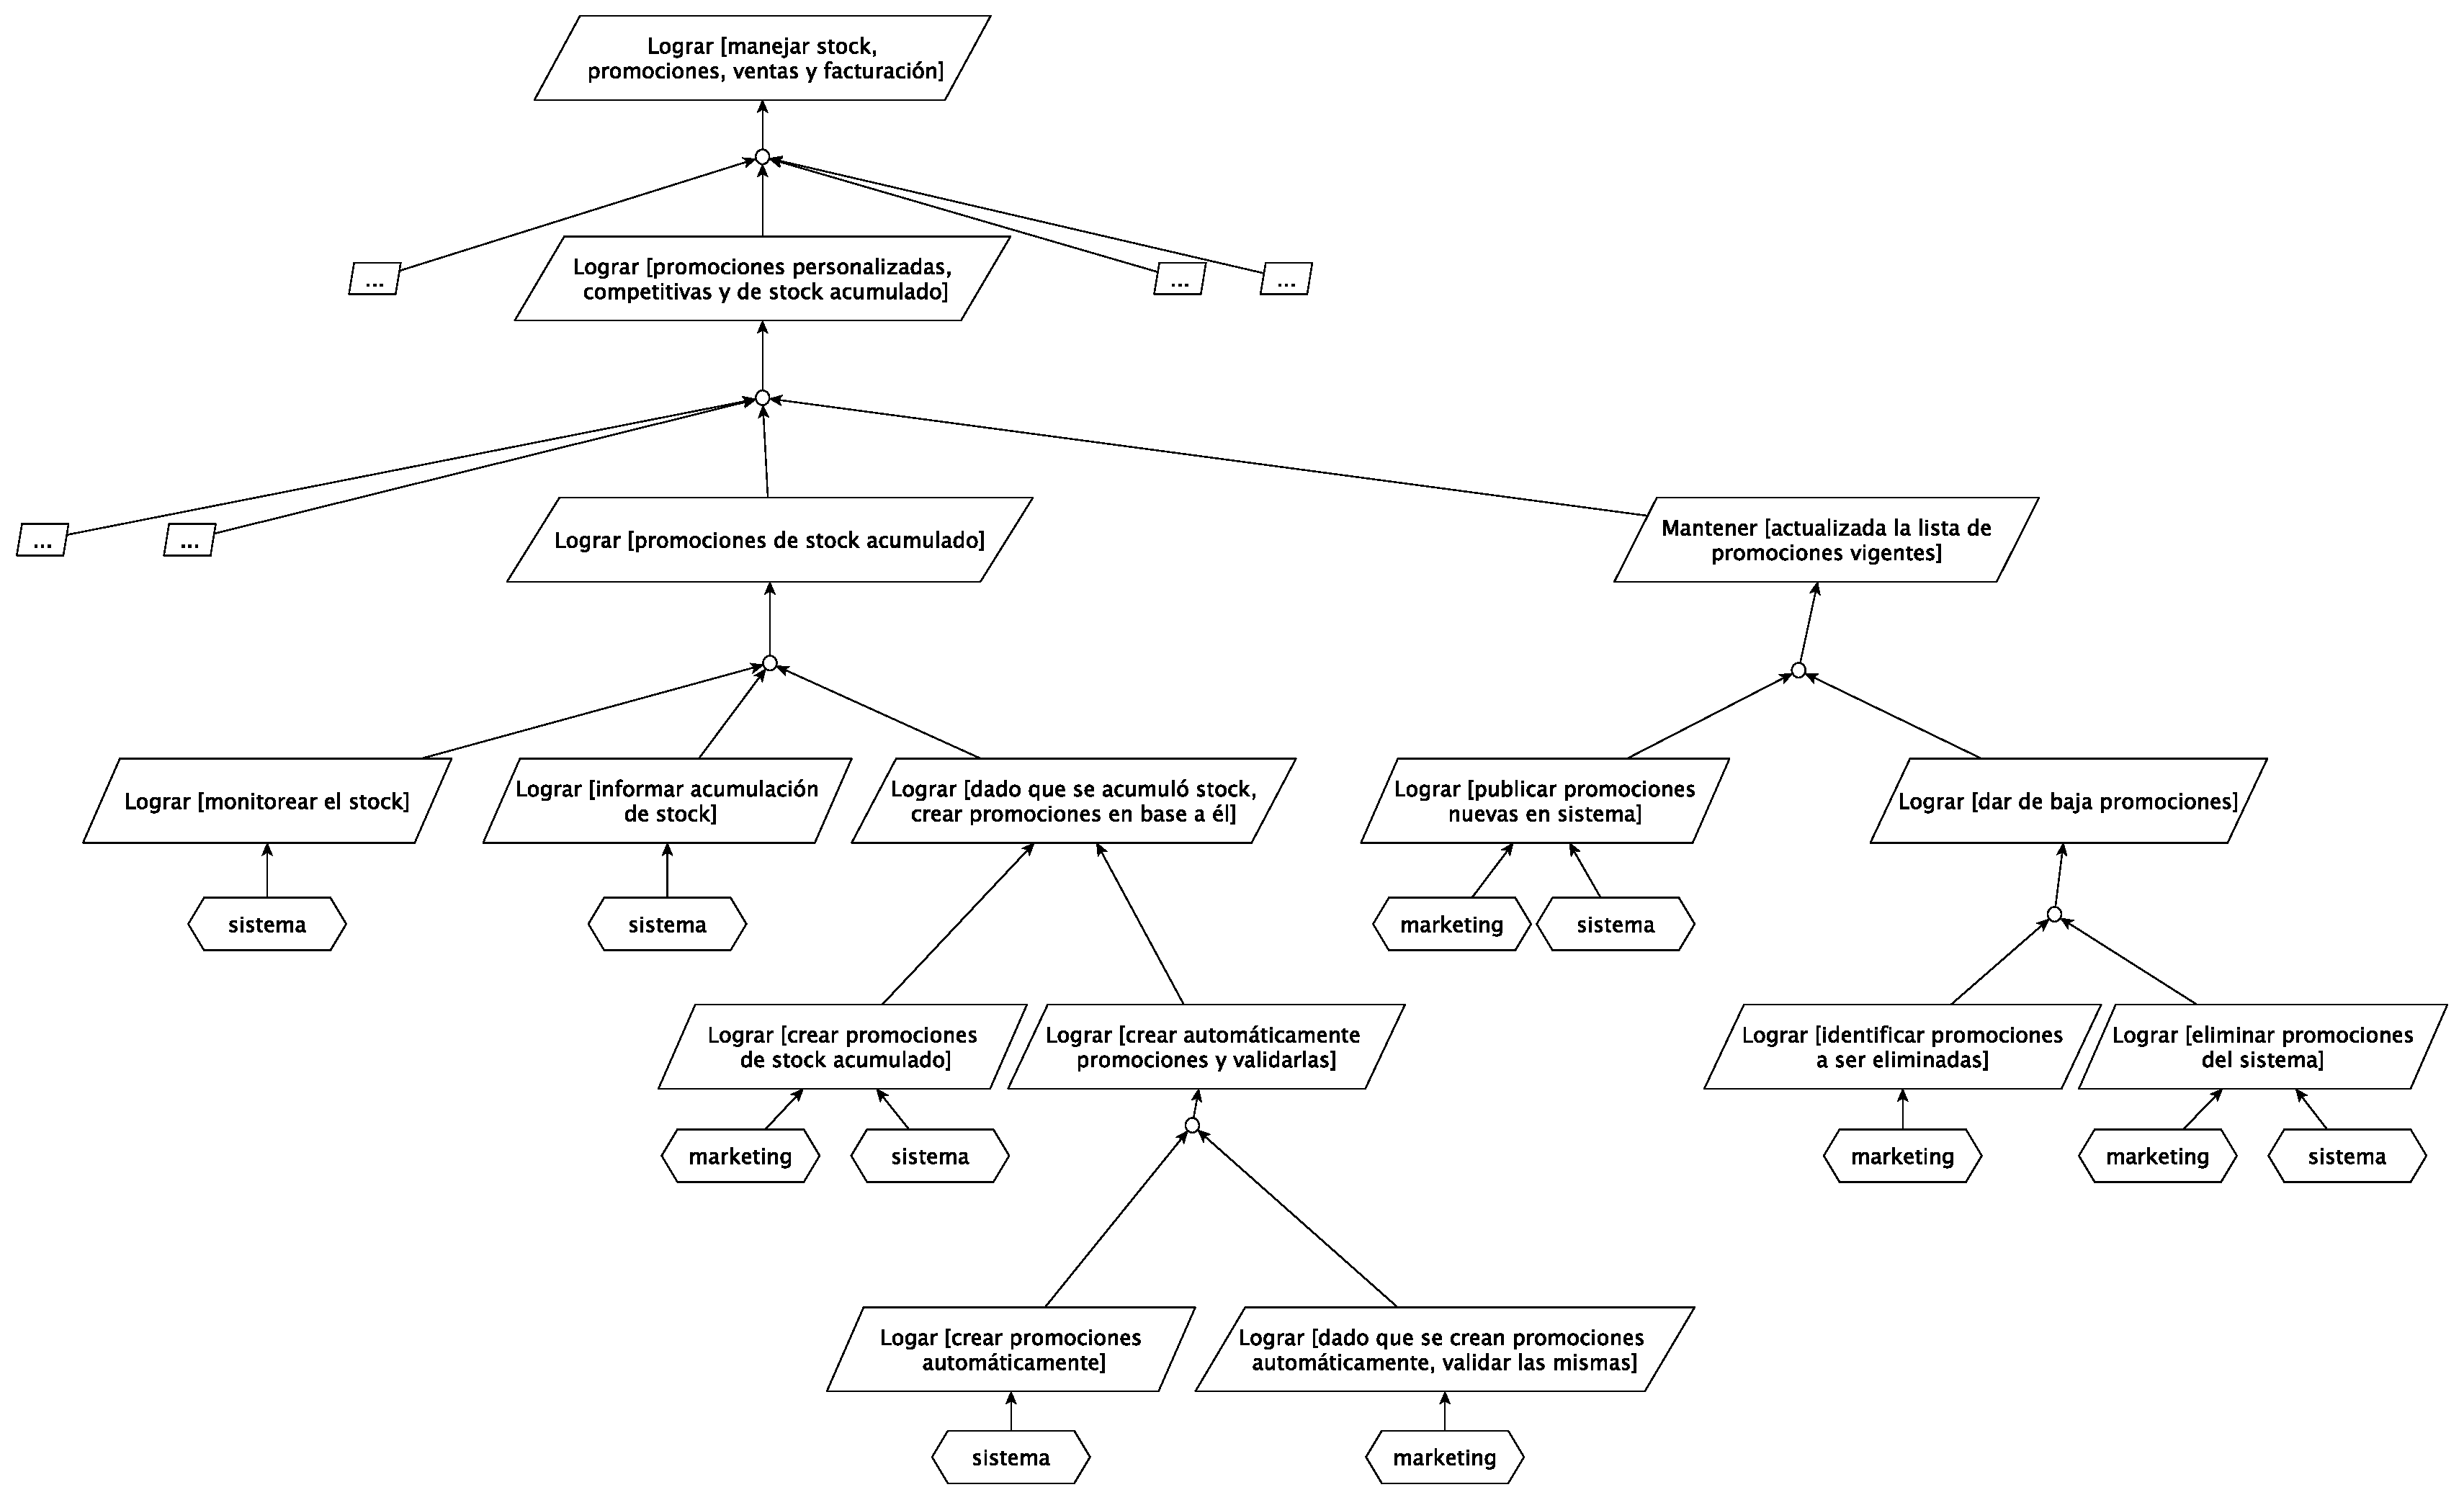
\includegraphics[width=1.3\textwidth, angle=90]{./imagenes/promociones_2.pdf}
  \caption{Diagrama de objetivos - Promociones (parte 2)}
  \label{fig:diagProm2}
\end{figure}

\clearpage

\subsection{Rama Ventas}

Nuestro sistema tiene como objetivo lograr realizar ventas personalizadas y confiables. Para lograr esto tenemos 6 objetivos a cumplir. A saber:
\begin{enumerate}
  \item Conocer los datos del cliente.
  \item Conocer las promociones disponibles para el mismo.
  \item Adaptar las promociones a necesidades particulares.
  \item Convencer al cliente de comprar una promoción.
  \item Reservar la misma.
  \item Confirmar la compra.
\end{enumerate}

\indent Para conocer los datos del cliente se debe averiguar, por un lado, la cantidad de líneas y la facturación mensual que posee en nuestra empresa, y por otro, las necesidades del mismo.\\
\indent El primer par de objetivos se puede obtener de dos formas: manteniendo los datos de los clientes a visitar en el dispositivo móvil del vendedor, actualizando diáriamente el dispositivo, o dándole la posibilidad de consultar los datos del cliente en el momento de forma inalámbrica.

\indent Asumiendo que ya conocemos los datos del cliente, queremos conocer que promociones tiene nuestra empresa para él. De manera similar a la anterior, tenemos la opción offline y la online. La offline consiste en mantener las promociones para los clientes a visitar en el dispositivo móvil del vendedor, actualizándo diariamente los datos de las promociones en el mismo. La opción online se basa en tener disponible las promociones para el cliente de manera inalámbrica. Un objetivo blando que nos planteamos es el de contar con las últimas promociones realizadas por marketing. La opción offline contribuye un poco a lograr esto, mientras que la online contribuye bastante, por poder tener disponibles las últimas generadas en el mismo día.\\
\\

% OJO! Acá hay 2 ramas que no tienen refinamiento. Es a propósito o nos falta?

\indent Nuestro sistema de ventas debe poder, luego que se adaptaron las promociones disponibles para el cliente a sus necesidades particulares y que se lo convenció de comprar una de las mismas, reservar una promoción.\\
\indent Para cumplir este objetivo se deben dar tres cosas:
\begin{enumerate}
  \item Se debe poder ingresar la promoción elegida, para lo cual necesitamos seleccionarla de una lista y enviarla al servidor.
  \item Se debe poder, dado que sucedió lo anteriormente dicho, comprobar la disponibilidad del stock para reservarla, manteniendo una conexión con el servidor (detalles sobre este objetivo más adelante).
  \item Se debe poder mantener actualizado el stock, dado que hubo disponibilidad para la reserva. Para esto debemos descontar el stock reservado y notificar al encargado si el stock está pronto a terminarse.
\end{enumerate}

\indent Por último, asumiendo que se cumplió lo anteriormente descripto, debemos lograr confirmar la compra. Esto se consigue logrando ingresar los datos del cliente necesarios para comprar, y enviándolos al servidor manteniendo la comunicación con el mismo.\\
\indent Hay dos formas de ingresar los datos del cliente necesarios para comprar: Se puede obtener los datos leyendo el código QR provisto por la AFIP de Cambodia, o se puede completar el formulario de facturación. Ambos contribuyen a disminuir el error humano, el primero por no necesitar de ninguna interacción al ingresar datos, y el segundo si bien requiere completar un formulario, es menos propenso a error que copiar datos de una tabla donde es fácil confundir las filas.\\

\indent El objetivo común que describimos como ``mantener comunicación con el servidor'' influye en cuatro objetivos blandos:
\begin{enumerate}
  \item Tener mayor performance.
  \item Tener disponible el servicio el mayor tiempo posible.
  \item Tener una comunicación segura.
  \item Reducir el costo de desarrollo y mantenimiento.
\end{enumerate}

Dicho objetivo común se puede lograr de dos maneras: mediante internet móvil o mediante envío y recepción de SMS. La forma en la que lo hace, es la siguiente:
\begin{itemize}
  \item Internet móvil: ayuda en gran parte al cumplimiento de los objetivos blandos 1 y 3, gracias a su velocidad y capacidad de encriptación. Ayuda también un poco al objetivo 4, y no consigue cumplir muy bien el 2, por lo planteado en el enunciado (el servicio es propenso a caerse).

  \item Envío y recepción de SMS: es una opción mala para el objetivo blando número 3, ya que no existe encriptación, y también para el objetivo 4. Es un poco peor que la alternativa de Internet móvil para el objetivo 1, y ayuda a cumplir el objetivo 2, ya que generalmente es un servicio que está disponible siempre.
\end{itemize}

\indent Para lograr comunicarse a través de internet, asumimos que el dispositivo móvil del vendedor tiene conexión a internet, y el mismo debe lograr enviar un pedido y recibir una respuesta. Para poder comunicarse a través de SMS, asumimos que el dispositivo cuenta con un chip GSM para conectarse a la red, y que nuevamente puede por este medio enviar un pedido y recibir una respuesta.

\subsubsection{Escenarios}

\begin{itemize}
  \item \textbf{Conocer los datos del cliente} \\
    Victor, el vendedor entra en las oficinas de Clelia \& Company, luego de la introducción comienza con su trabajo consultando al sistema la cantidad de líneas y facturación del cliente y a su vez al cliente sus necesidades. El sistema puede obtener los datos de alguna de las dos maneras, o bien consulta al servidor a través de internet o bien responde con los datos cargados al iniciar el día laboral.

  \item \textbf{Conocer y Adaptar las promociones para el cliente} \\
    Victor, luego de conocer las necesidades del cliente, utiliza su dispositivo para obtener las promociones que se ajustan a las necesidades del cliente y demás promociones creadas por el departamento de Marketin. Una vez más, el sistema puede obtener los datos de alguna de las dos maneras, o bien consulta al servidor a través de internet o bien responde con los datos cargados al iniciar el día laboral. Victor, como excelente vendedor, utiliza sus habilidades para incrementar la venta adaptando las promociones al cliente.
    No sólo es hábil para adaptar las promociones sino que también logra convencer al cliente de concretar la venta.

  \item \textbf{Reservar una promoción} \\
    Víctor y Virginia, ambos vendedores en clientes diferentes, cierran una venta cada uno sobre la misma
    promoción. Ambos envían el formulario de confirmación de una promoción desde sus dispositivos móviles.

    La solicitud de Víctor se procesa primero, quien recibe del sistema la
    notificación de que su promoción ha sido reservada. Luego de esto, el stock
    es insuficiente como para realizar otra venta de ese estilo. Al momento que
    llega al sistema el pedido de Virginia, el sistema le notifica que no puede
    realizarse la operación y que la promoción está deshabilitada por falta de
    stock.

  \item \textbf{Confirmar la compra} \\
    Luego de que Víctor recibió la notificación de que el stock para su 
    promoción está disponible ingresa en su dispositivo móvil los datos del cliente necesarios para la factura (mediante el formulario o leyendo un código 
    QR), la tarjeta de crédito y los números que el cliente desea para las líneas nuevas uno a uno. 
    Finalmente envía el formulario al servidor.
\end{itemize}


\begin{figure}[h!]
  \centering
  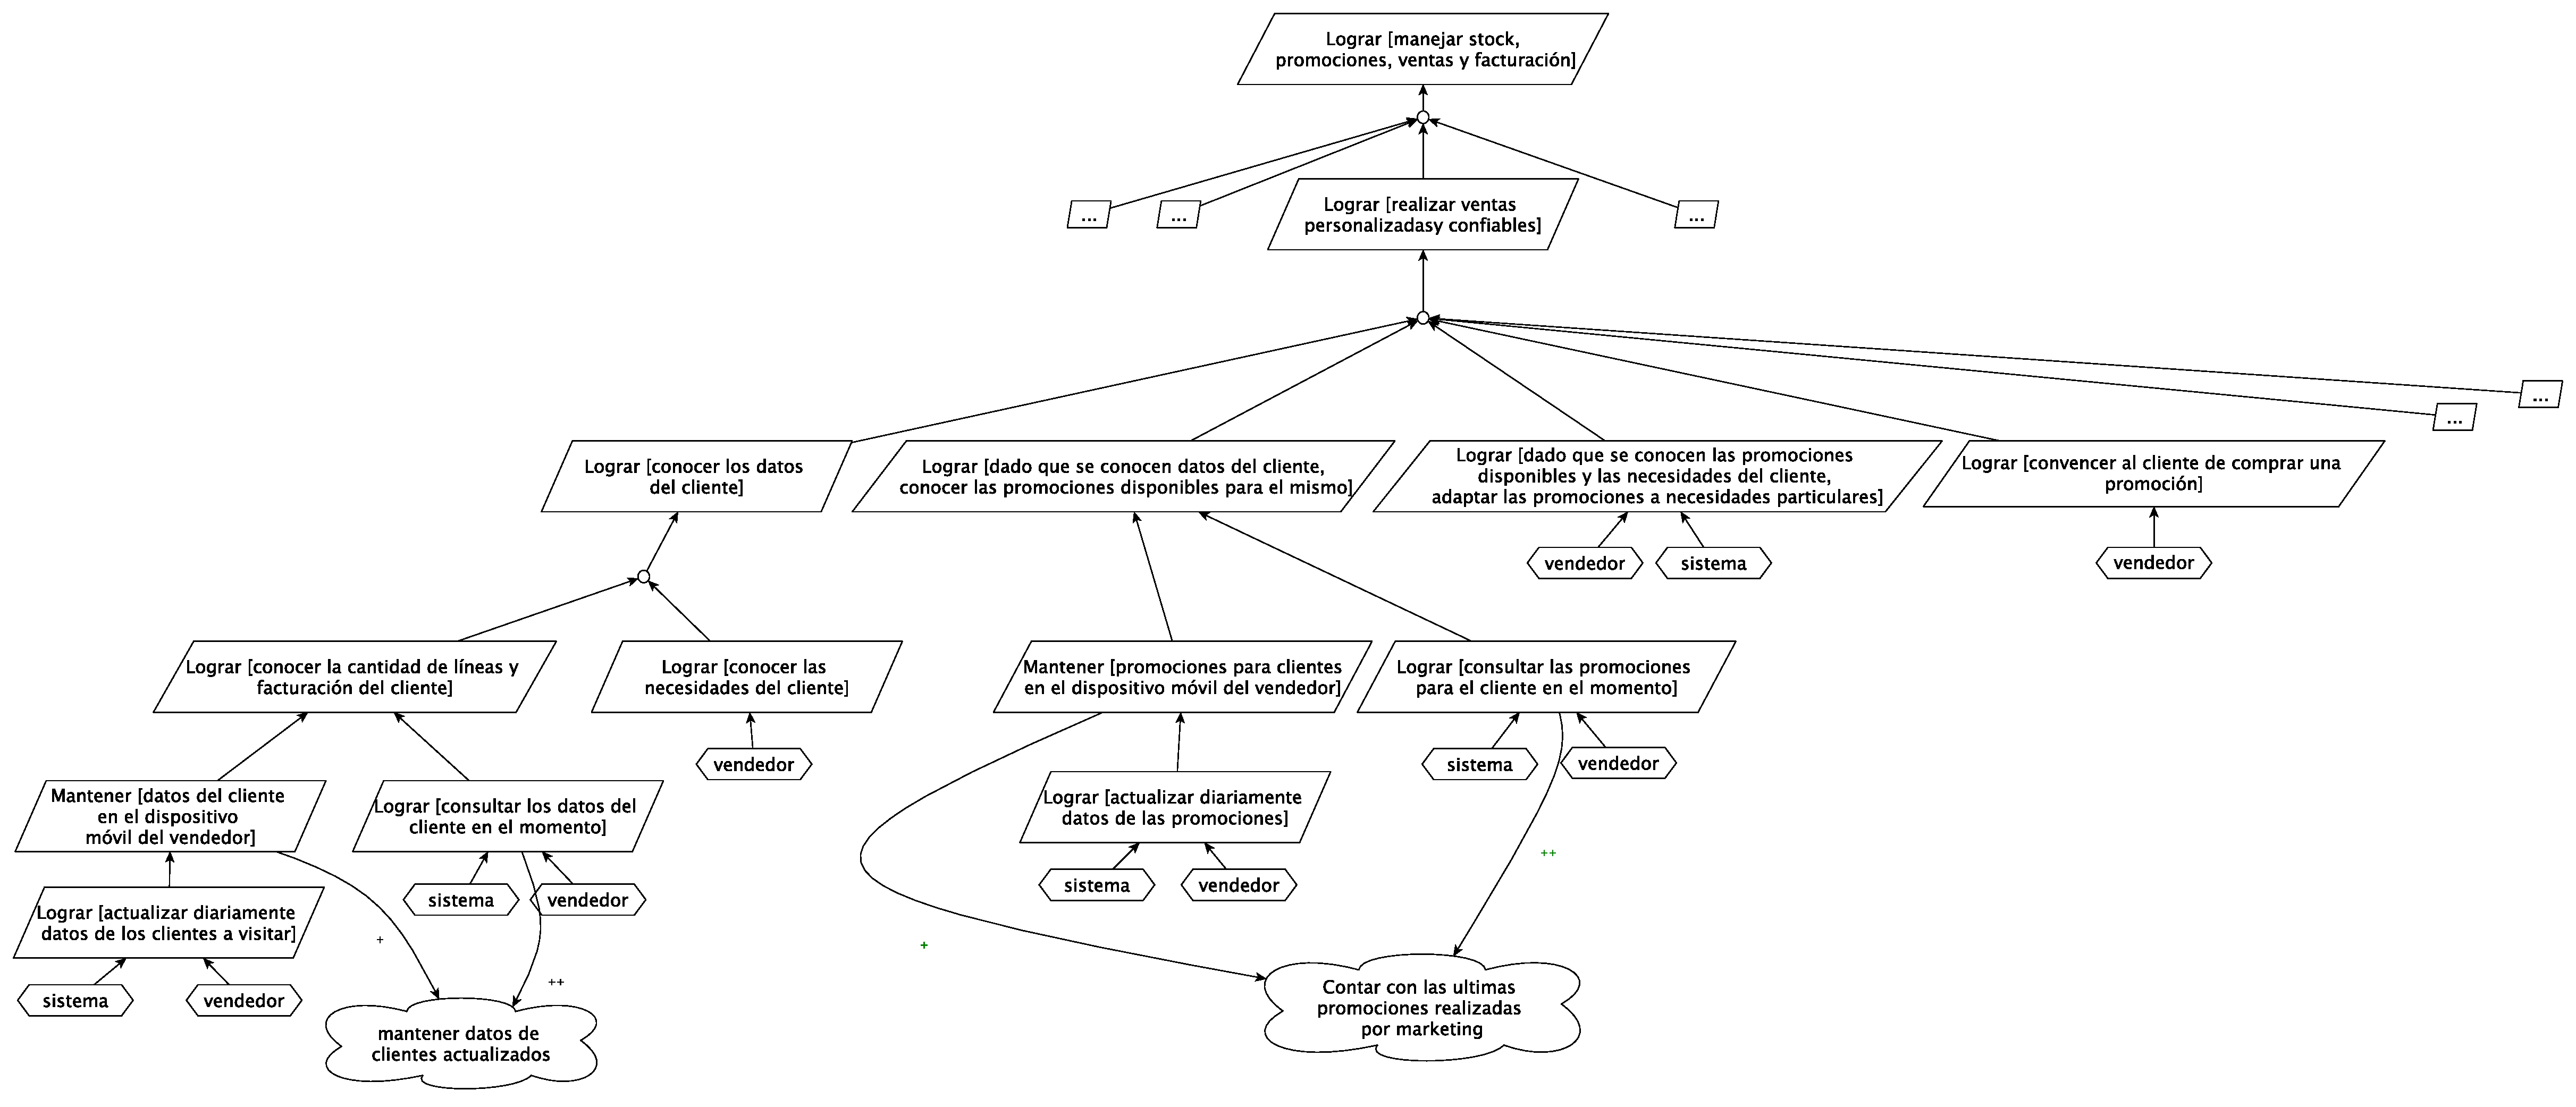
\includegraphics[width=1.5\textwidth, angle=90]{./imagenes/ventas_1.pdf}
  \caption{Diagrama de objetivos - Ventas (parte 1)}
\end{figure}


\clearpage

\clearpage

\begin{figure}[h!]
  \centering
  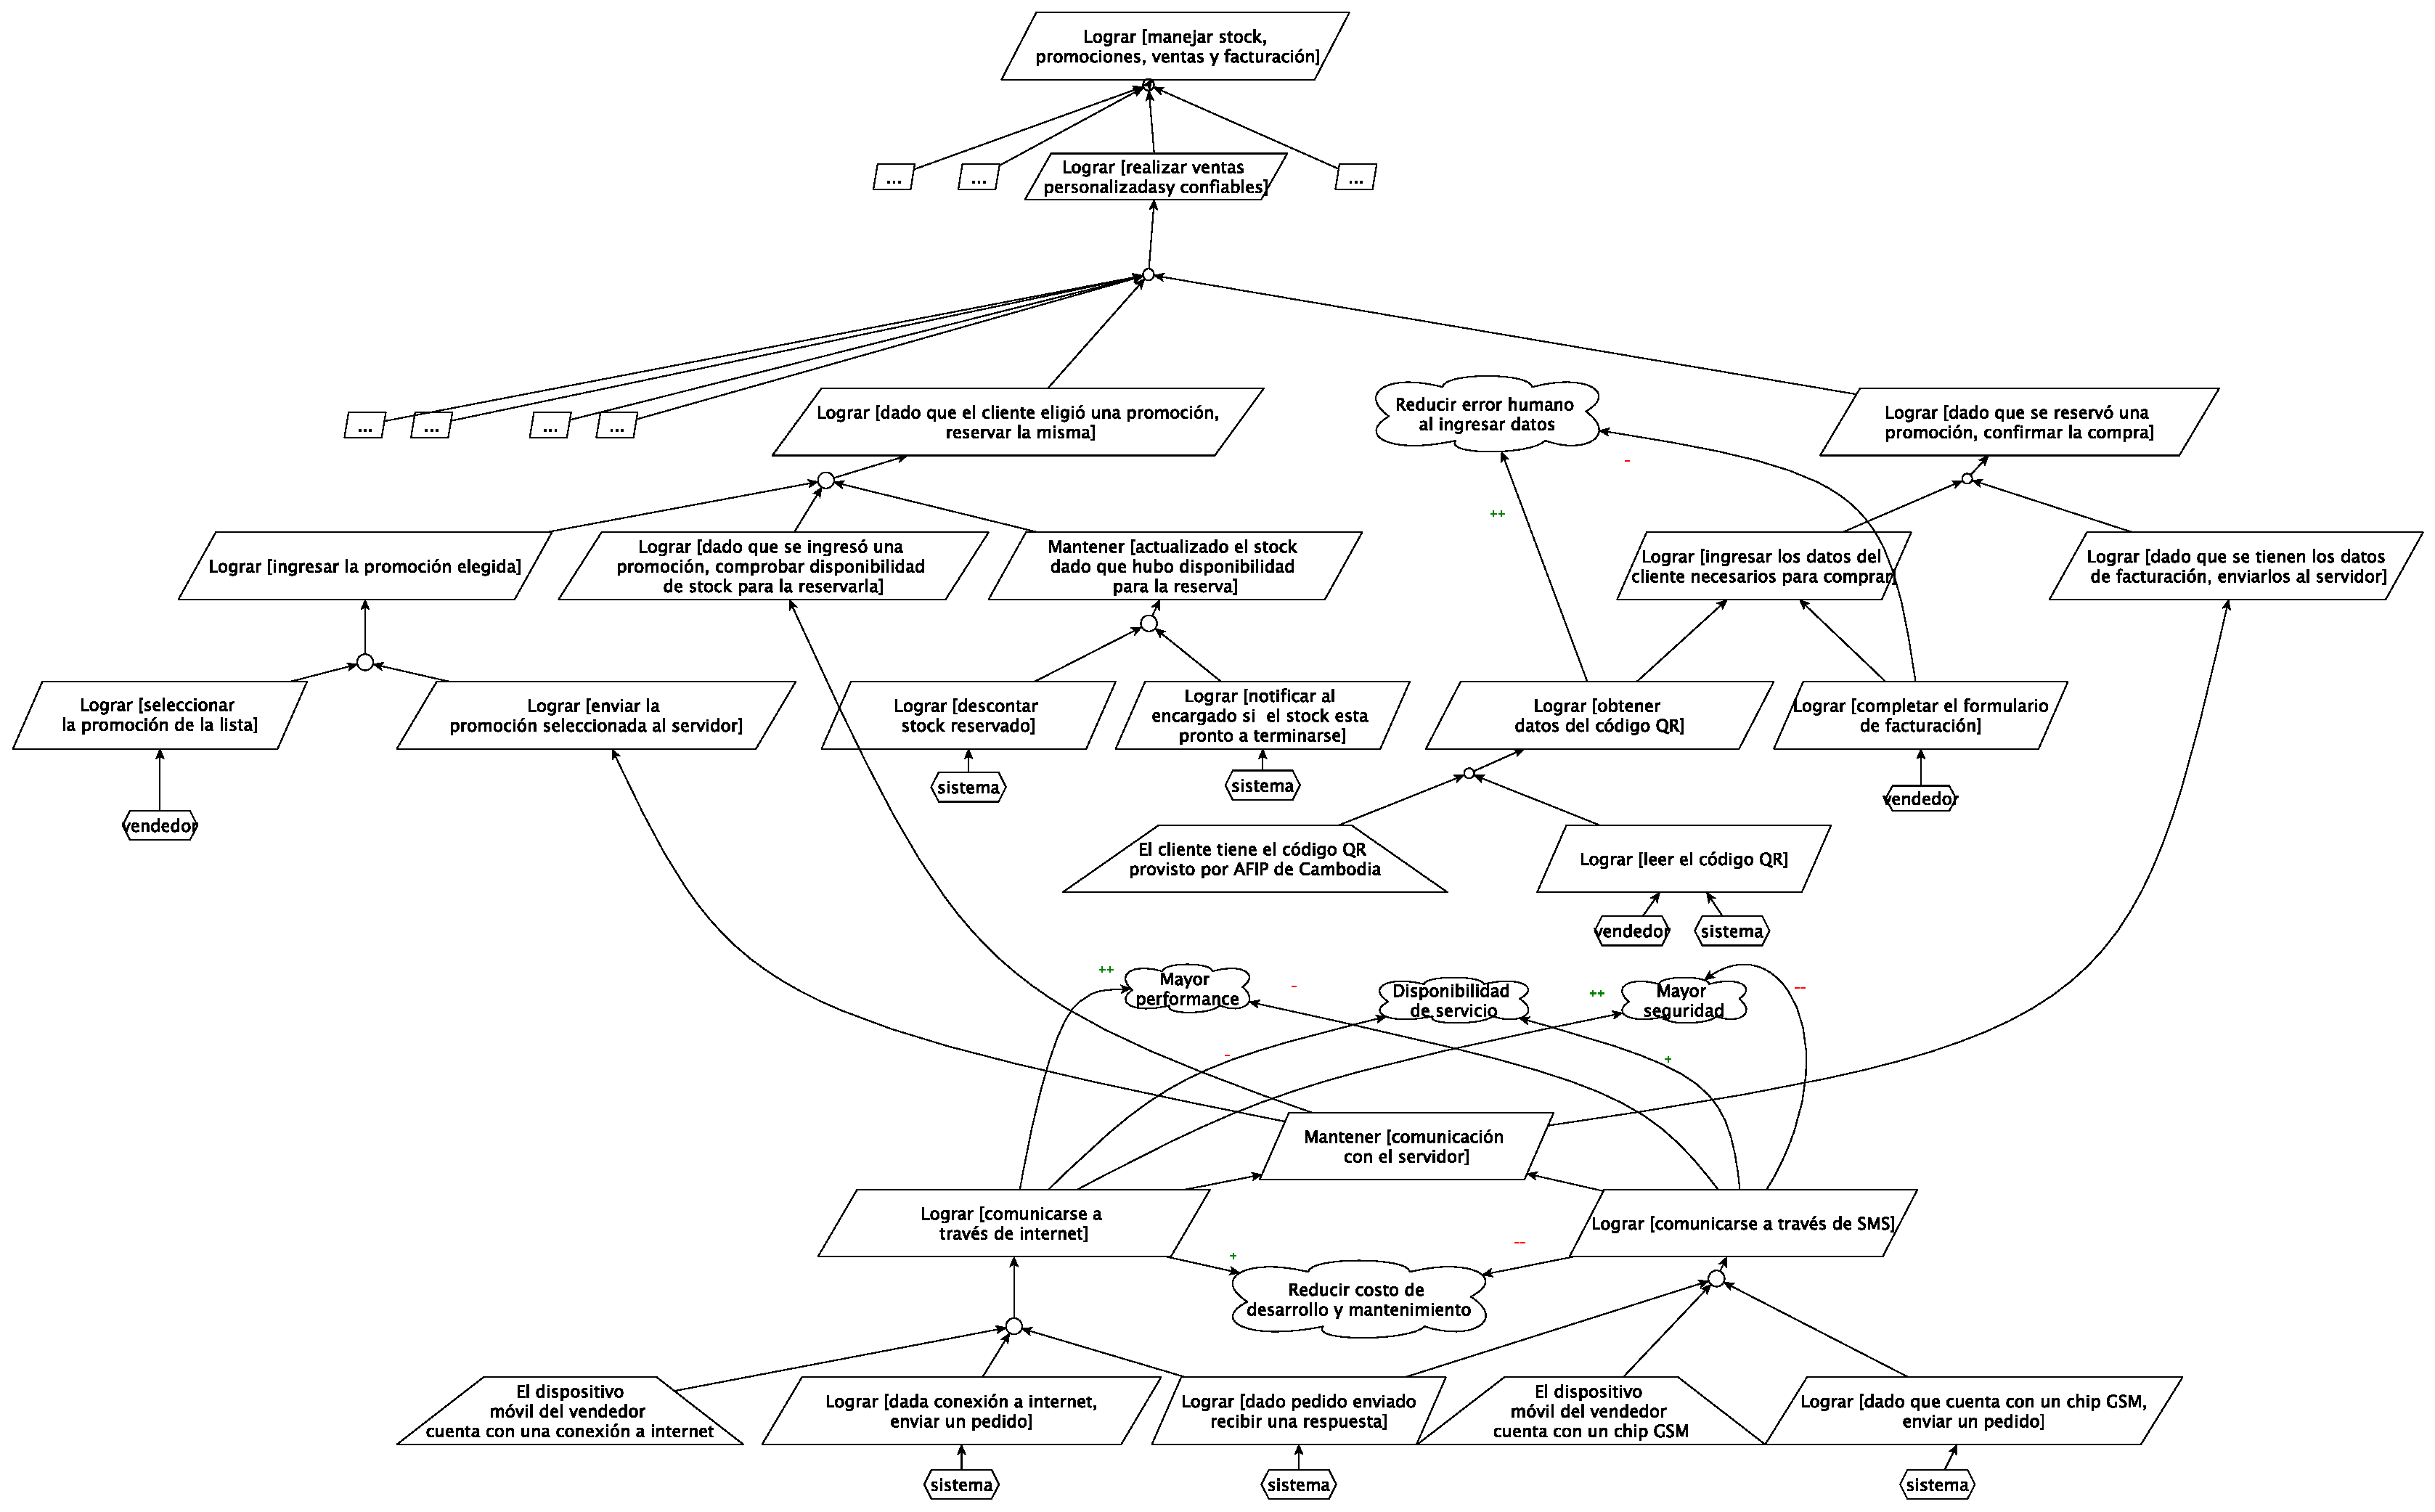
\includegraphics[width=1.5\textwidth, angle=90]{./imagenes/ventas_2.pdf}
  \caption{Diagrama de objetivos - Ventas (parte 2)}
\end{figure}

\clearpage

\subsection{Rama Facturacion}

Finalmente, el último pilar sobre el que se apoya la satisfacción del objetivo principal del sistema es el de facturación. En este aspecto se busca una facturación confiable, lo más automatizada posible a partir de las ventas y que no introduzca errores que enlentezcan el proceso de entrega de equipos a los clientes. Para esto, el departamento de facturación recibe la notificación de las ventas realizadas instantáneamente al haber sido realizadas por los vendedores. Luego, deberá proceder a verificar los datos del cliente y chequear que todo esté en regla, lo cual dependerá explícitamente de los estándares de control implementados por el departamento. Una vez que facturación valide al cliente podrá confirmar la venta a través del sistema, lo cual disparará una notificación al encargado de stock para que se ocupe de armar y coordinar la entrega. Por otro lado, facturación deberá seguir más allá y, utilizando los datos digitalmente provistos por el sistema de ventas, realizar la facturación correspondiente en su sistema externo para tal fin. De cualquier manera se garantizará que haya compatibilidad entre ambos sistemas con el objetivo de que los empleados de facturación no necesiten reingresar ningún dato de manera manual y así poder reducir posibles errores en la etapa final del proceso.

\subsubsection{Escenarios}

\begin{itemize}
  \item \textbf{Confirmar o Rechazar una venta} \\
    Luego que Victor cerró la venta con el cliente, el sistema notifica al departamento de Facturación para proceder con la verificación del estado del Cliente. 
    Fernando, del departamento de facturación verifica que el cliente sea apto 
    para realizar negocios con él bajo el protocolo que corresponda (Veraz, AFIP de Cambodia, etc) 
    y luego utilza nuestro sistema para realizar una de dos acciones:
  \begin{itemize}
    \item \textbf{Confirmar venta de cliente verificado} \\
      Confirma la venta en el sistema que notifica inmediatamente al encargado de Stock que los equipos pueden ser retirados.
    \item \textbf{Rechazar venta de cliente verificado} \\
      Rechaza la venta en el sistema que notifica inmediatamente al encargado de Stock que los equipos no deben ser retirados hasta que no se solucione el problema o vuelvan a estar disponibles.
  \end{itemize}

  \item \textbf{Facturar los equipos y líneas} \\
    Fernando selecciona las ventas confirmadas a facturar y las exporta en un formato compatible con el sistema de Facturación. La integración entre estos sistemas optimiza el tiempo de Fernando y reduce los errores que éste podría cometer.
\end{itemize}

\begin{figure}[h!]
  \centering
  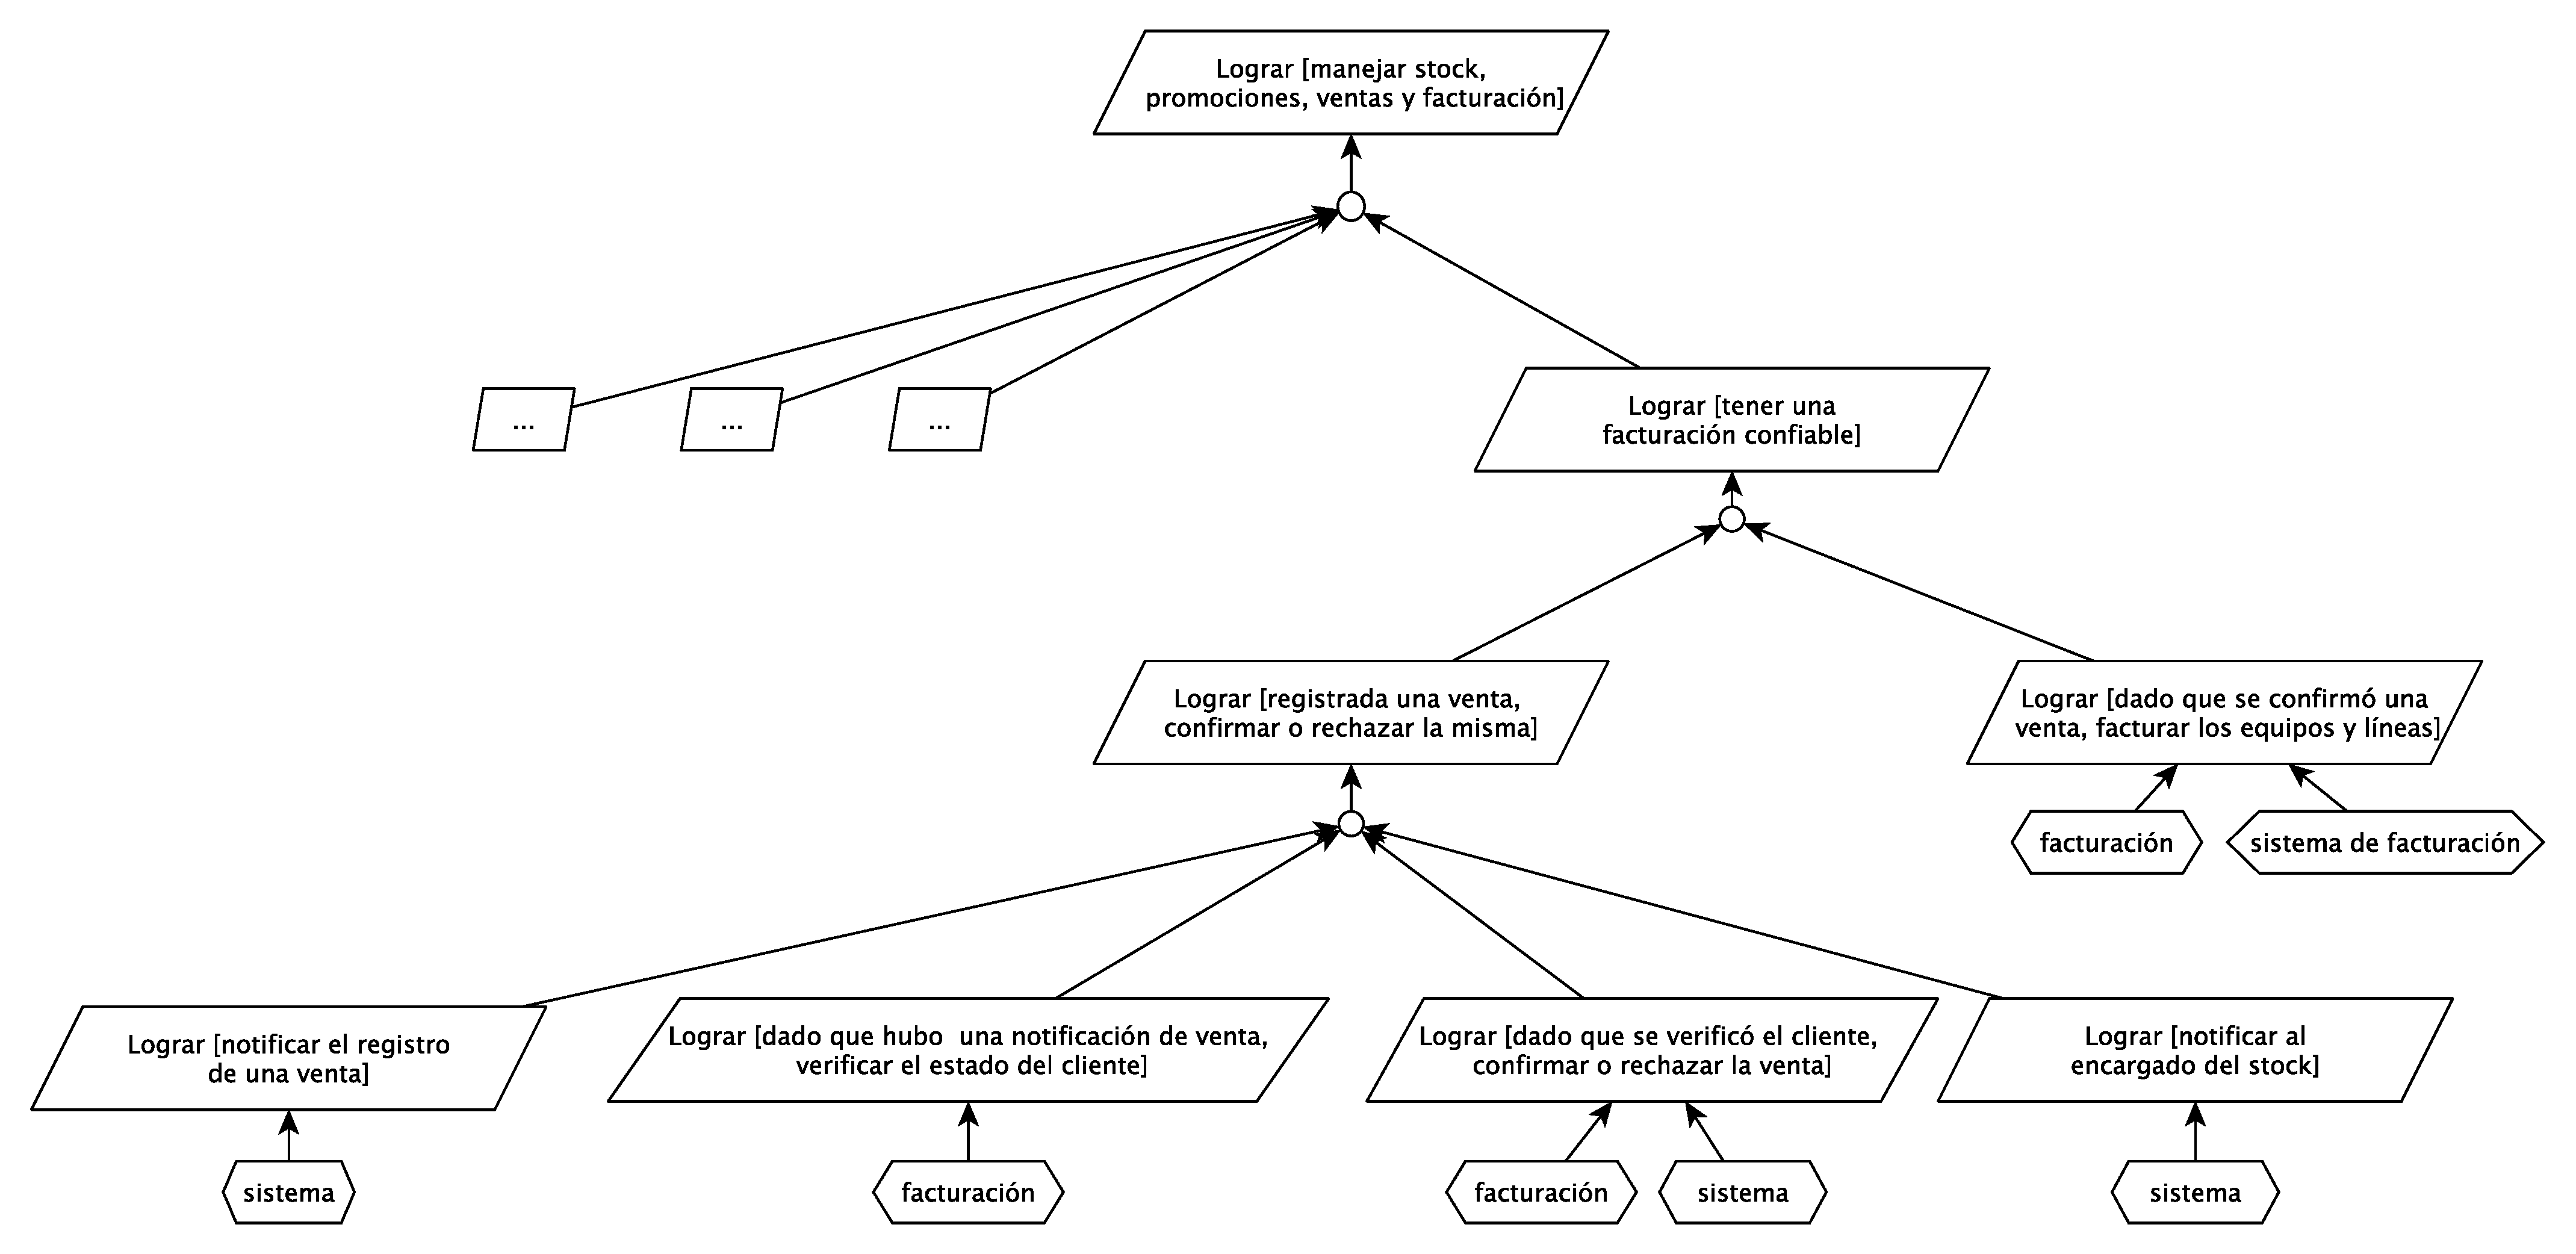
\includegraphics[width=1\textwidth]{./imagenes/facturacion.pdf}
  \caption{Diagrama de objetivos - Facturacion}
\end{figure}

